\documentclass{article}

\usepackage{xeCJK}
\usepackage{hyperref}
\usepackage{cite}
\usepackage{geometry}
\usepackage{amsmath}
\usepackage{indentfirst}
\usepackage{algorithm}
\usepackage{algorithmic}
\usepackage{graphicx}

\linespread{2}%修改行距
\setlength{\parindent}{2em}


\begin{document}

\title{通信客户流失预警模型数据挖掘报告}
\author{介应奇}
\date{\today}
\maketitle
\tableofcontents


\section{业务背景}
使用分类模型构建客户流失预测模型,通过客户为流失客户的概率预测该客户是否为流失客户并根据客户为流失客户的概率生成流失概率排序名单。

\section{数据理解}
在本案例中使用的数据来自于IBM Sample Data Sets,是某电信公司一段时间内的客户消费数据。共包含7043笔客户资料,每笔客户资料包含21个字段,其中1个客户ID字段,19个属性特征字段及1个标签字段(Yes代表流失,No代表未流失)。属性特征字段主要包含以下三个维度指标:客户画像指标(如性别、是否老年等)、消费产品指标(如是否开通互联网服务、是否开通电话服务等)、消费信息指标(如付款方式、月费用等)。字段的具体说明如表 1所示:

\section{数据准备}
这里的数据准备包含了一共5个部分,数据导入,数据清理,数据选择与变换,数据平衡性改善,数据压缩。
这其中数据导入、数据清理、数据转换是公用模块,在后续的实验中的数据都是经过了这些共同的步骤,
至于数据的平衡性改善和数据压缩模块产生的数据并不会替换原有的数据,而是用新的变量记录下来了不同情况
处理的值,方便后续的对比分析,下面呈现代码处理的过程以及说明。

\subsection{数据导入}
\begin{figure}[H]
	\centering
	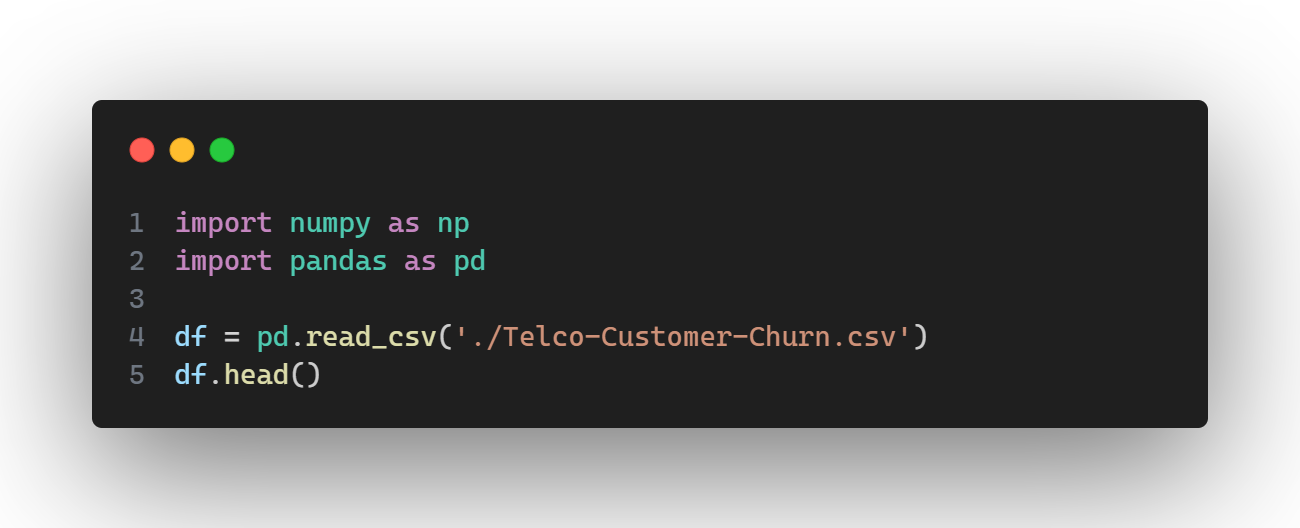
\includegraphics[width=\textwidth]{./img/import_data.png}
\end{figure}

\subsection{数据清理}
首先进行初步的数据清洗工作,包含错误值和异常值处理,并识别字段类型。其中清洗工作主要包含:
\begin{itemize}
	\item 对MultipleLines(是否开通多线服务)、OnlineSecurity(是否开通网络安全服务)、OnlineBackup(是否开通在线备份业务)、DeviceProtection(是否开通了设备保护业务)、TechSupport(是否开通了技术支持服务)、StreamingTV(是否开通网络电视)、StreamingMovies(是否开通网络电影)等属性特征进行错误值处理。如不满足前置条件,则这些特征直接取值为No(若未开通互联网服务,自然不会开通网络电视等服务)。
	\item 对TotalCharges(总费用)特征进行异常值处理。将空白取值替换空值nan,由于含空值的行较少,将其一并删除。删除后该特征取值只有数值,因此将此特征类型设为浮点型。
	\item 判断字段的类别
\end{itemize}
数据清洗代码如下所示:
\begin{figure}[H]
	\centering
	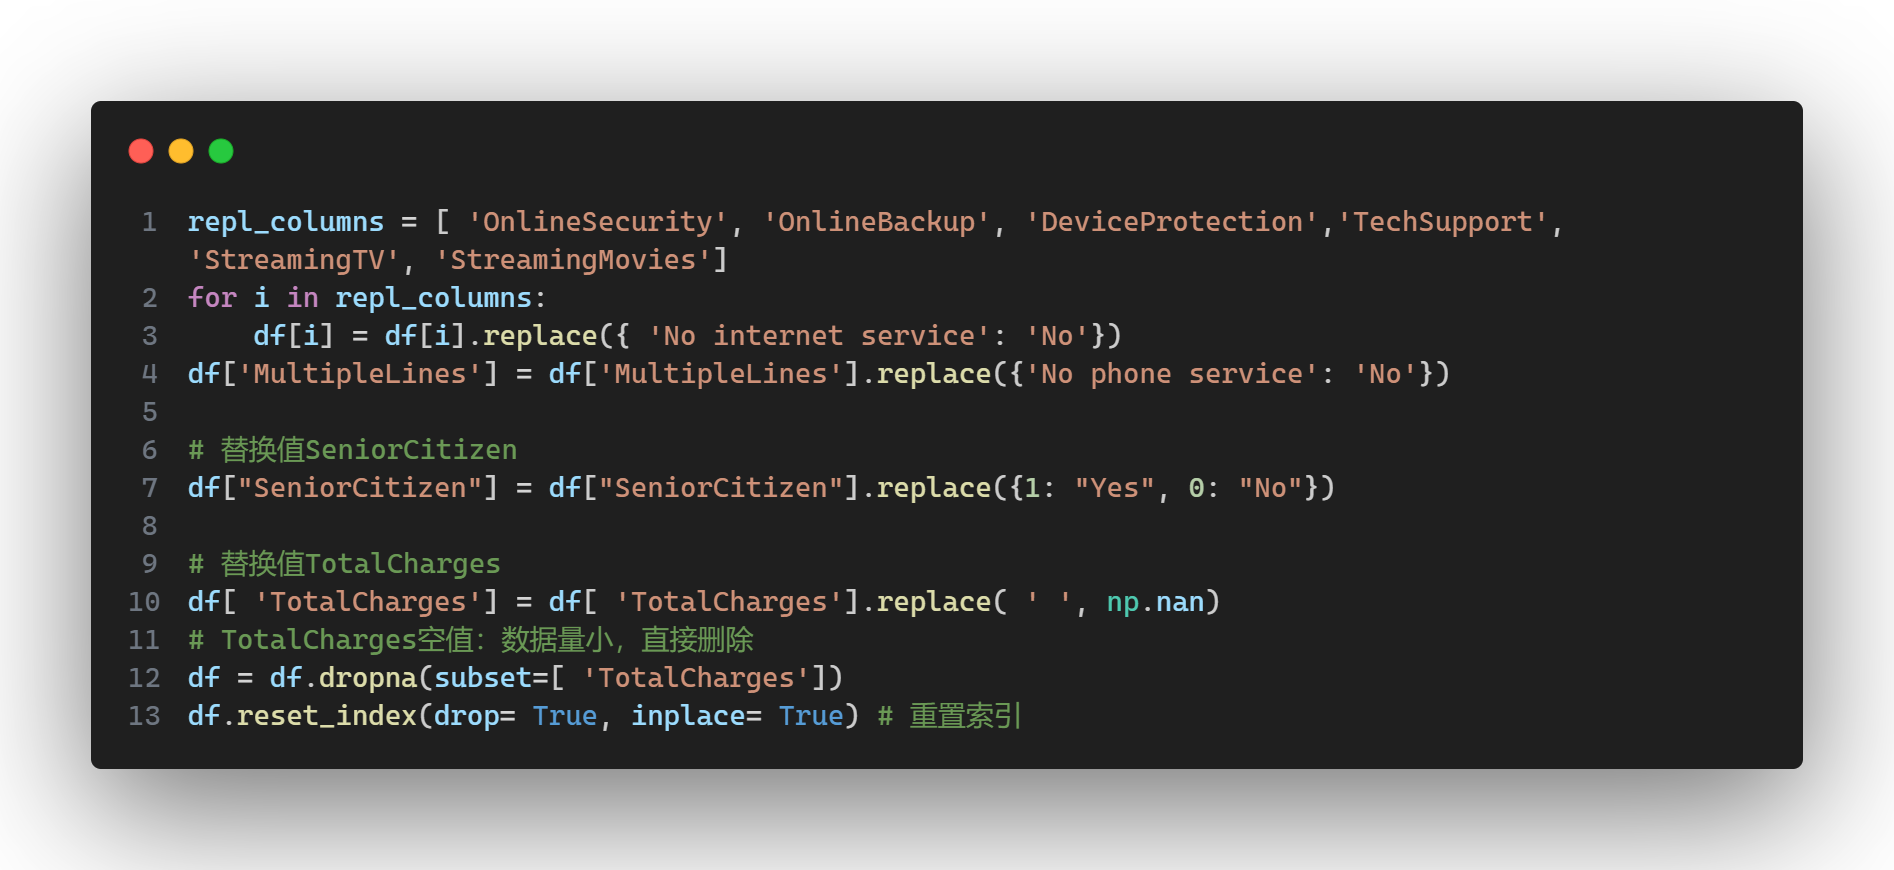
\includegraphics[width=\textwidth]{./img/data_clean.png}
\end{figure}

\subsection{数据选择与变换}
\subsubsection{数据选择}
区分离散和连续变量

\begin{figure}[H]
	\centering
	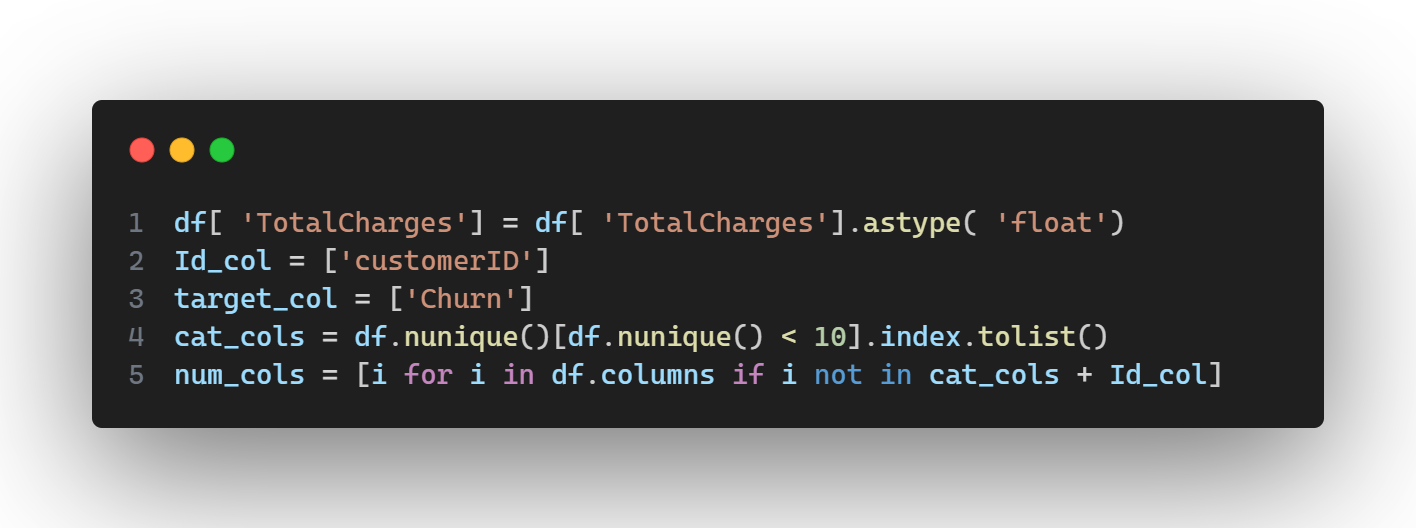
\includegraphics[width=\textwidth]{./img/data_select.png}
\end{figure}

\subsubsection{数据转换}

\begin{figure}[H]
	\centering
	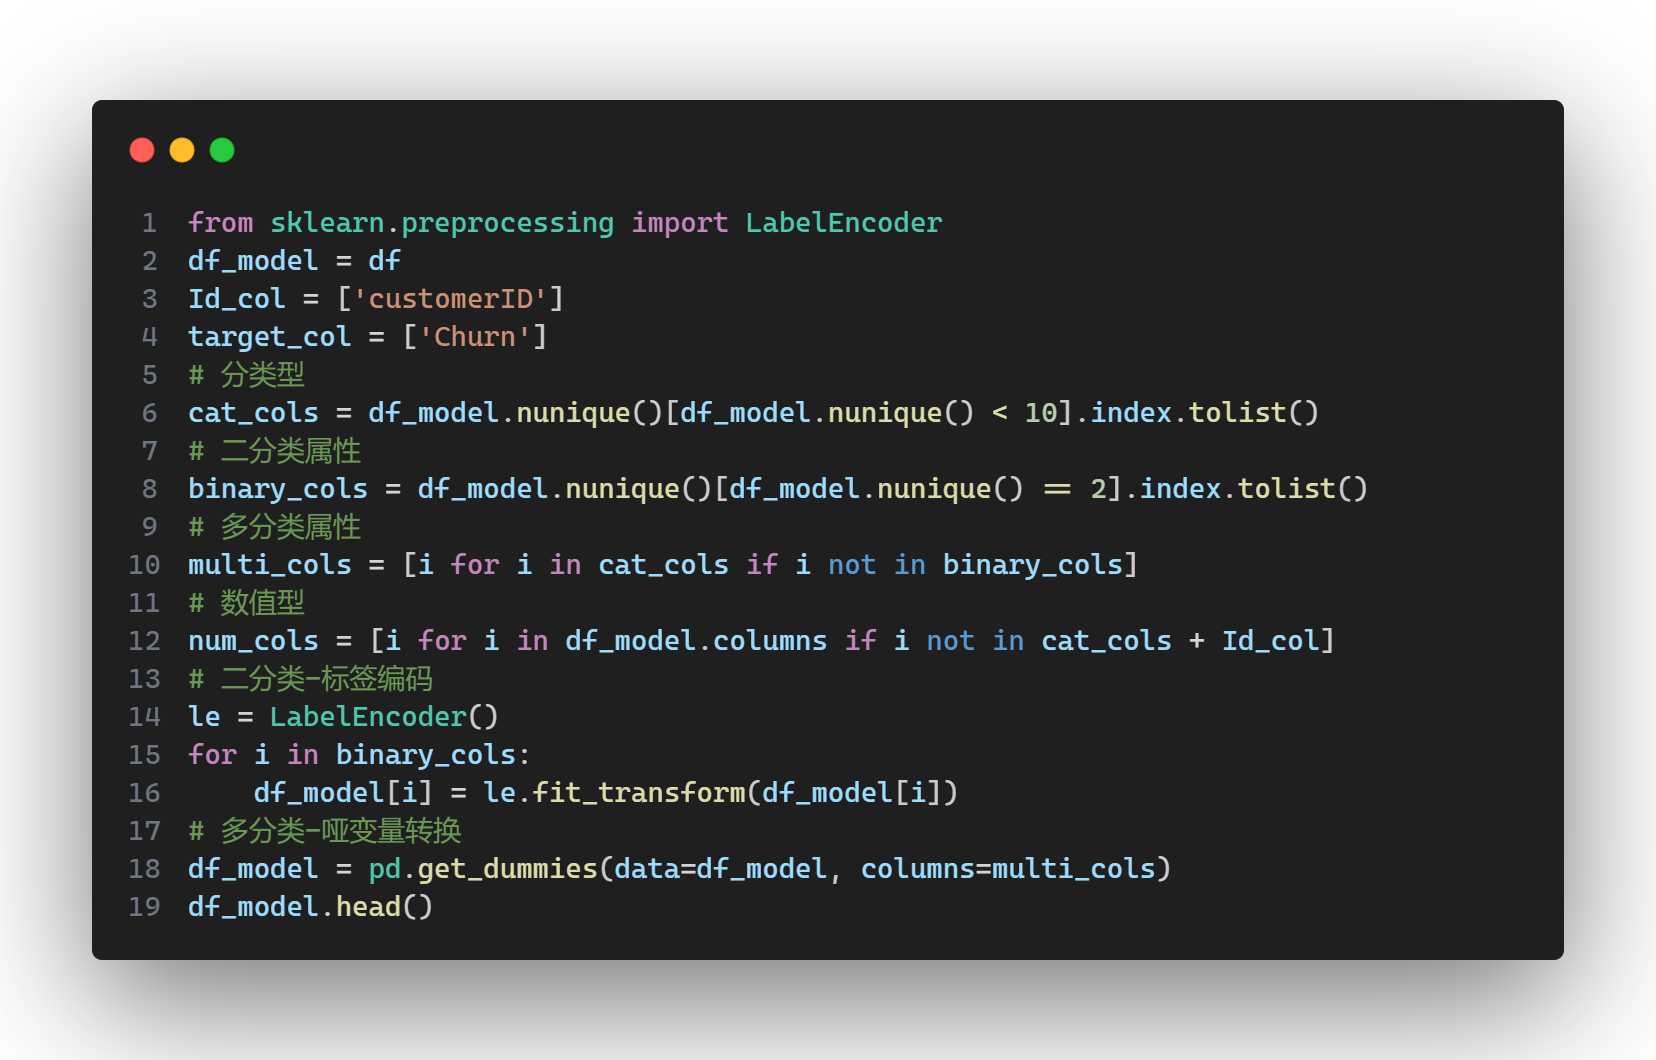
\includegraphics[width=\textwidth]{./img/data_transform.png}
\end{figure}

将转换后的数据定义为自变量和标签值

\begin{figure}[H]
	\centering
	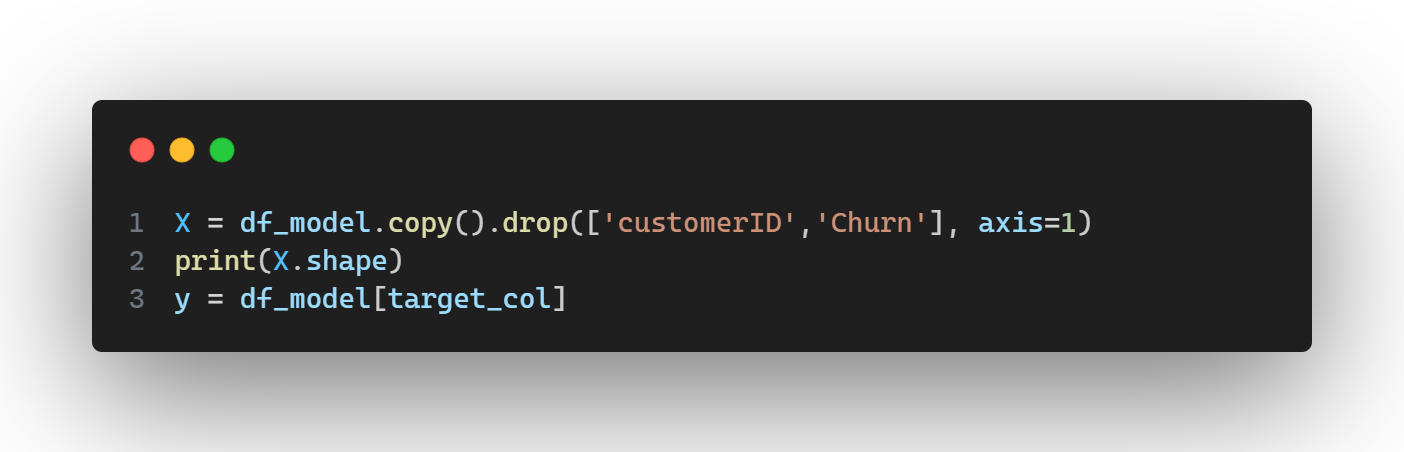
\includegraphics[width=\textwidth]{./img/x_y.png}
\end{figure}
这个数据是没有经过特征筛选的,因为不是所有的模型都需要经过特征筛选才能使用,有一些的特征选择是在模型中自己隐形选择的,因此我们在这里要保留一份最完整特征版的数据

\subsubsection{数据归一化}
保证模型能够快速收敛,并且消除数据的属性之间阈值不一致的差异性

满足python建模需要,需要对数据做以下处理。
•	对于分类变量,编码为0和1;
•	对于多分类变量,进行哑变量转换;
对于数值型变量,部分模型如KNN、神经网络、Logistic需要进行标准化处理。

\begin{figure}[H]
	\centering
	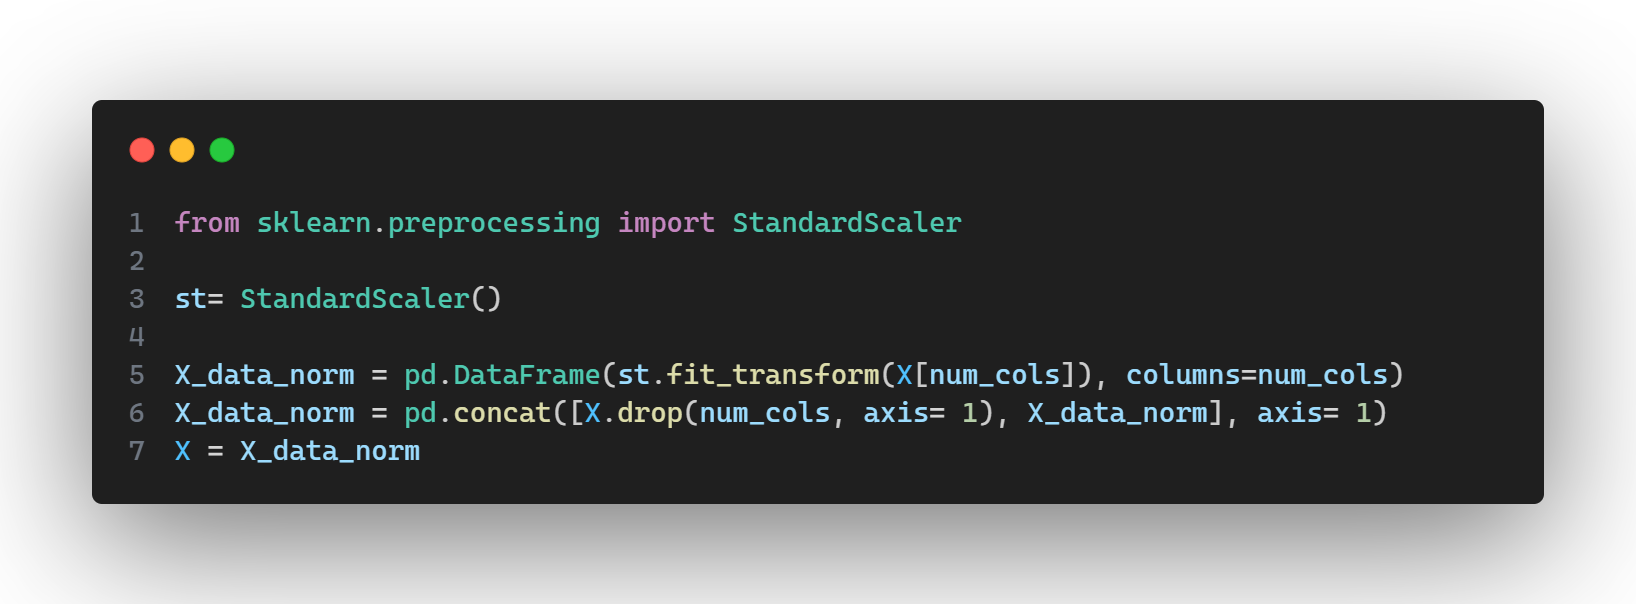
\includegraphics[width=\textwidth]{./img/normal.png}
\end{figure}

\subsection{数据平衡性改善}
因为我们发现流失客户和未流失客户的样本数量是不平衡的,因此使用上采样的方式增加流失客户的数据量从而使数据平衡性得到改善

\begin{figure}[H]
	\centering
	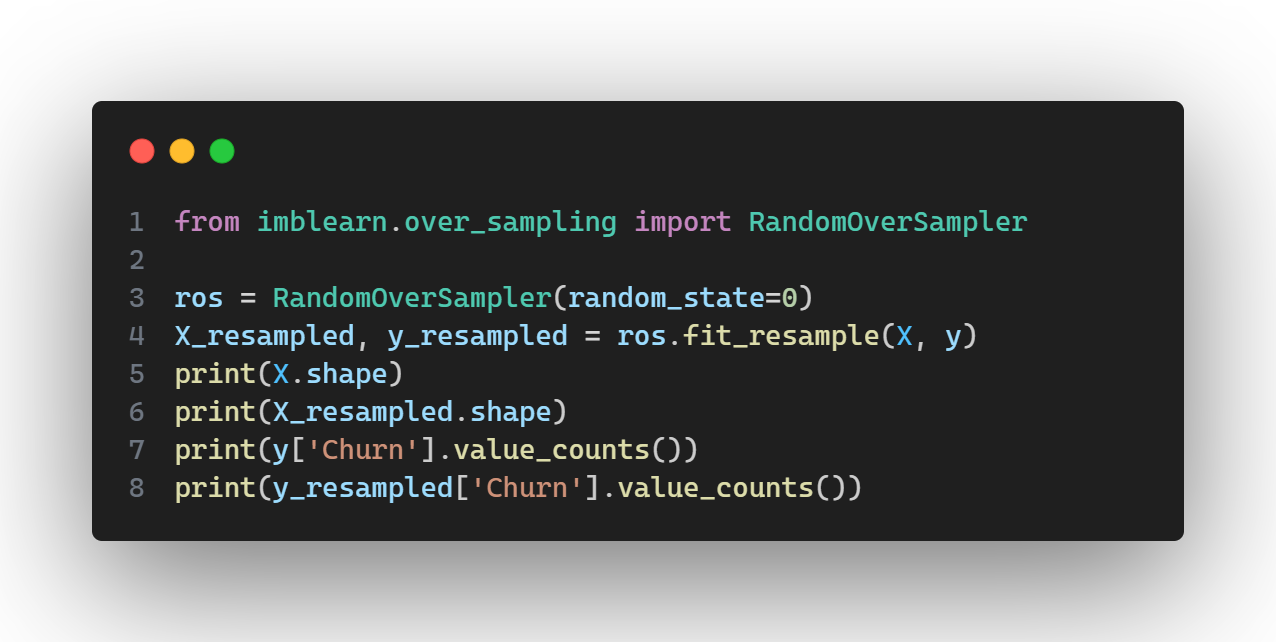
\includegraphics[width=\textwidth]{./img/resample.png}
\end{figure}

观察上述记过我们可以看到经过上采样之后,我们的y对应的两种标签值的数据数量一致了,具体观察对应的y值分布变化可以看出来是将流失客户数据进行了补齐,补齐到了和未流失客户数据两相同的程度


\subsection{数据压缩}

\subsubsection{PCA主成分分析法对数据实现不同程度的无监督压缩}

\begin{figure}[H]
	\centering
	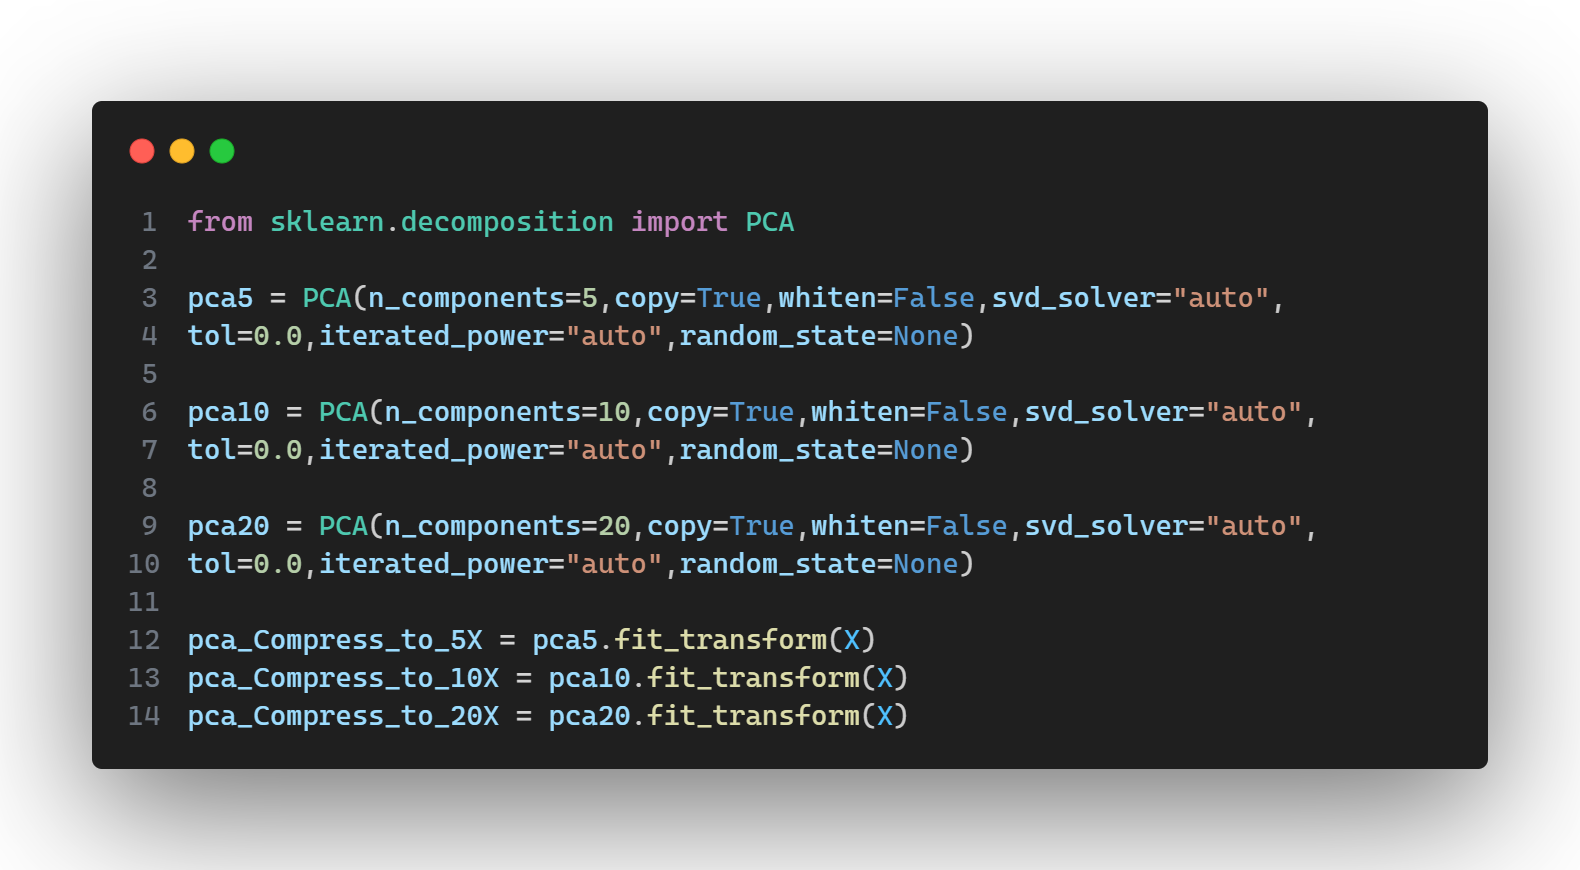
\includegraphics[width=\textwidth]{./img/pca_comp.png}
\end{figure}
通过pca方法我获取到了保留了维度值分别为5/10/20的自变量

\subsubsection{使用特征检定的方式进行特征筛选}

\begin{figure}[H]
	\centering
	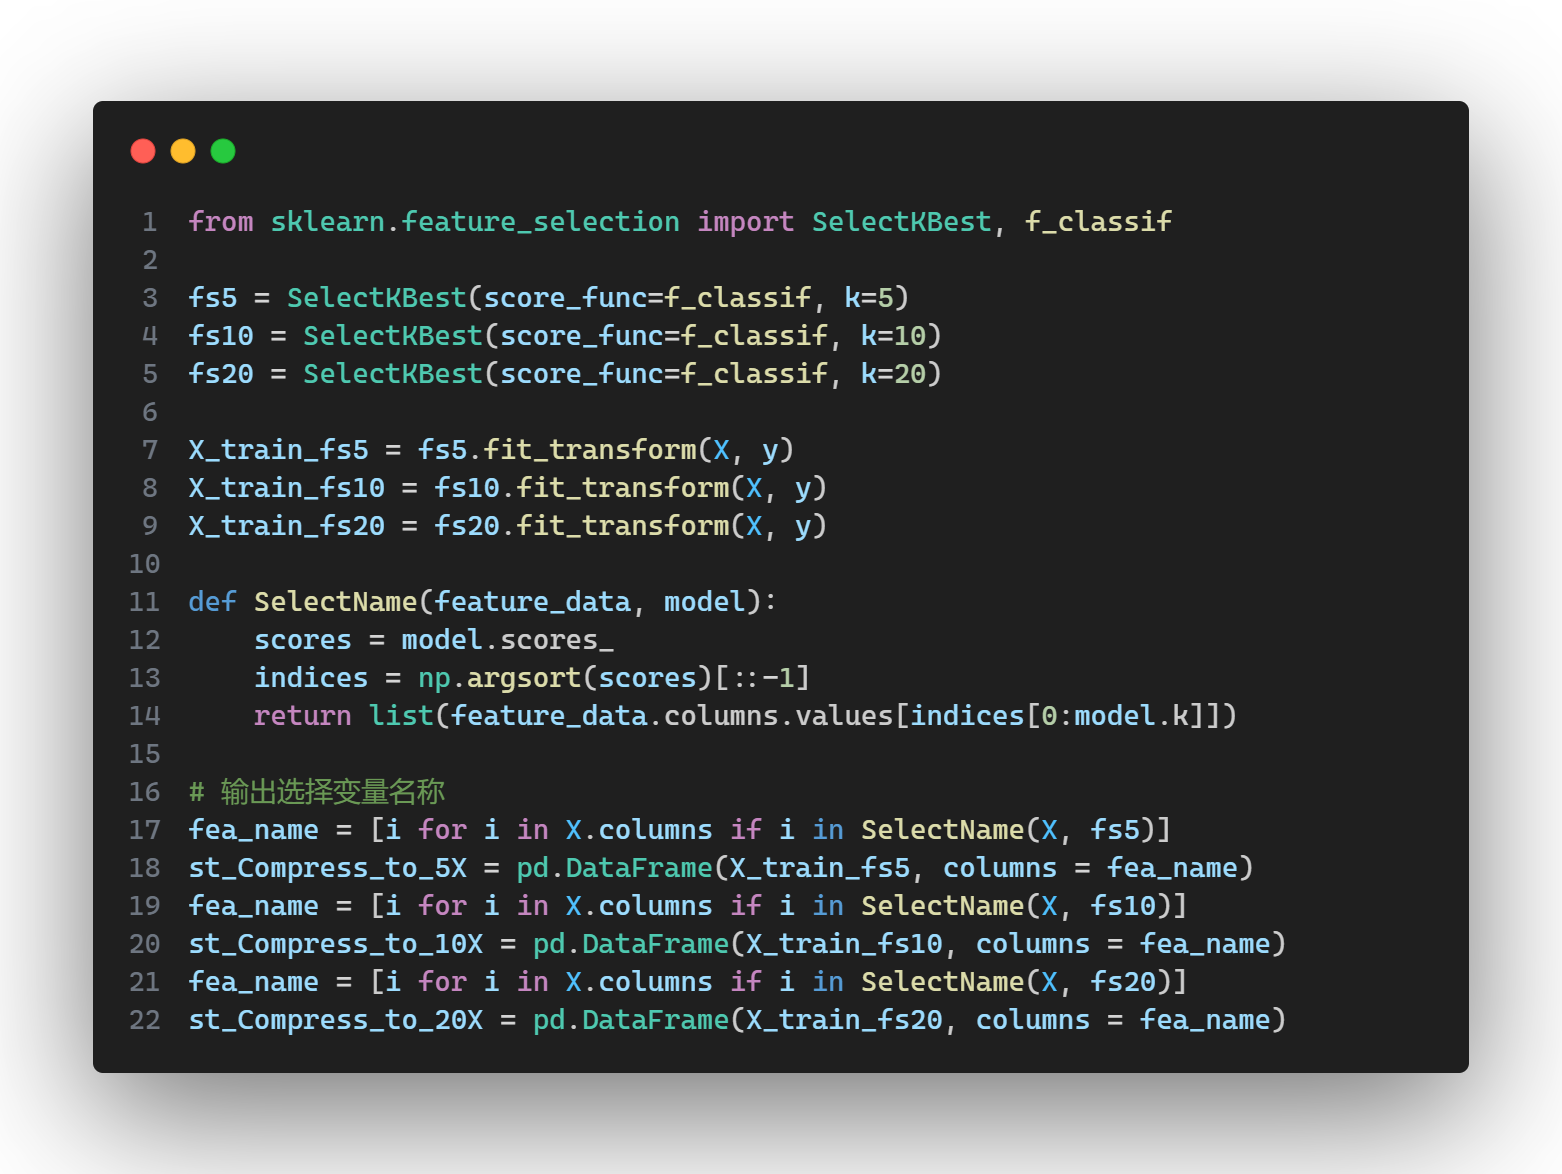
\includegraphics[width=\textwidth]{./img/fs_comp.png}
\end{figure}
通过特征检定的方法我获取到了保留了维度值分别为5/10/20的自变量

\section{探索性分析}
对指标进行归纳梳理,分用户画像指标,消费产品指标,消费信息指标。探索影响用户流失的关键因素。
首先查看流失用户与非流失用户的整体分布情况。
\begin{figure}[H]
	\centering
	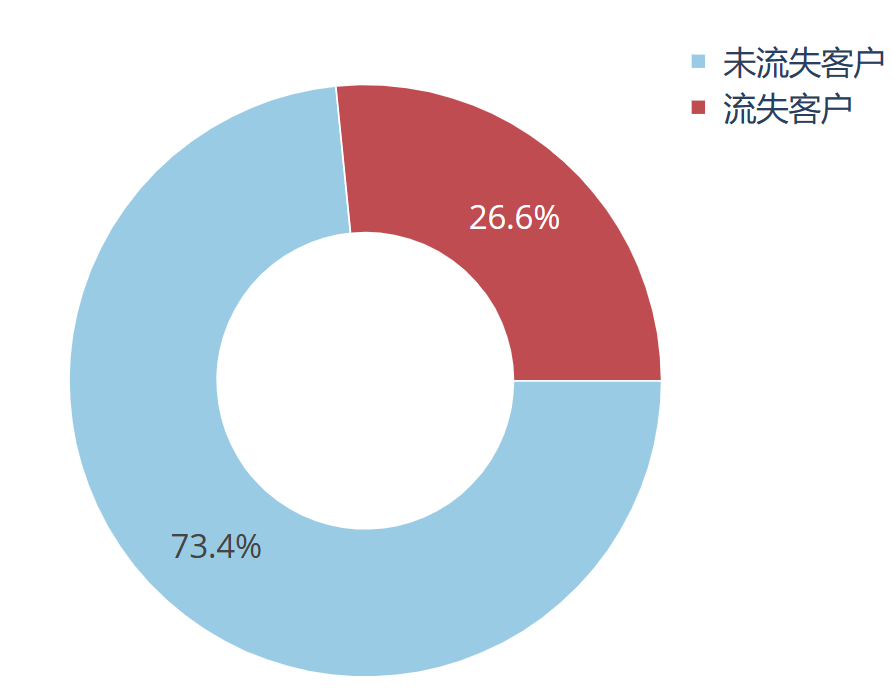
\includegraphics[width=\textwidth]{./img/t1.png}
\end{figure}
可以看出,经过初步清洗之后的数据集大小为7032条记录,其中流失客户为1869条,占比26.6%,未流失客户占比73.4%。
再分别探索对各特征的影响。
将每一个变量不同取值条件下用户流失与否用柱形图表示出来,可以直观地看出变量取值是否影响用户流失。

\begin{figure}[H]
	\centering
	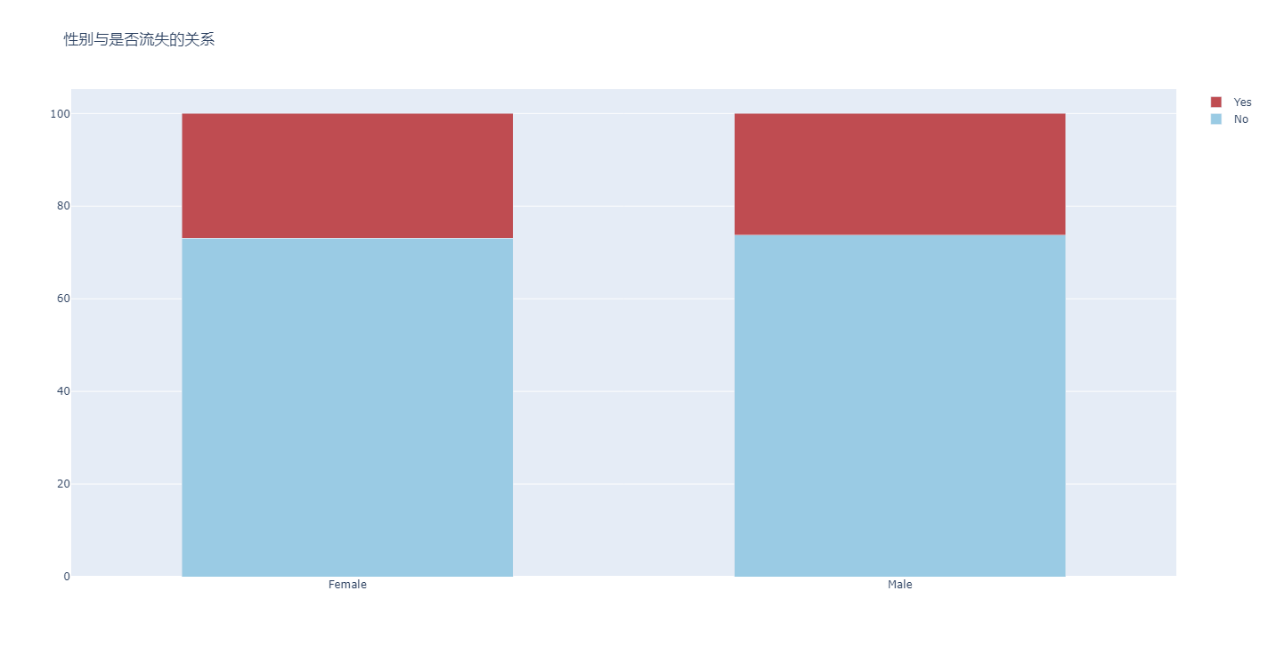
\includegraphics[width=\textwidth]{./img/t2.png}
\end{figure}
可以看出,男性和女性在客户流失比例上没有显著差异。

\begin{figure}[H]
	\centering
	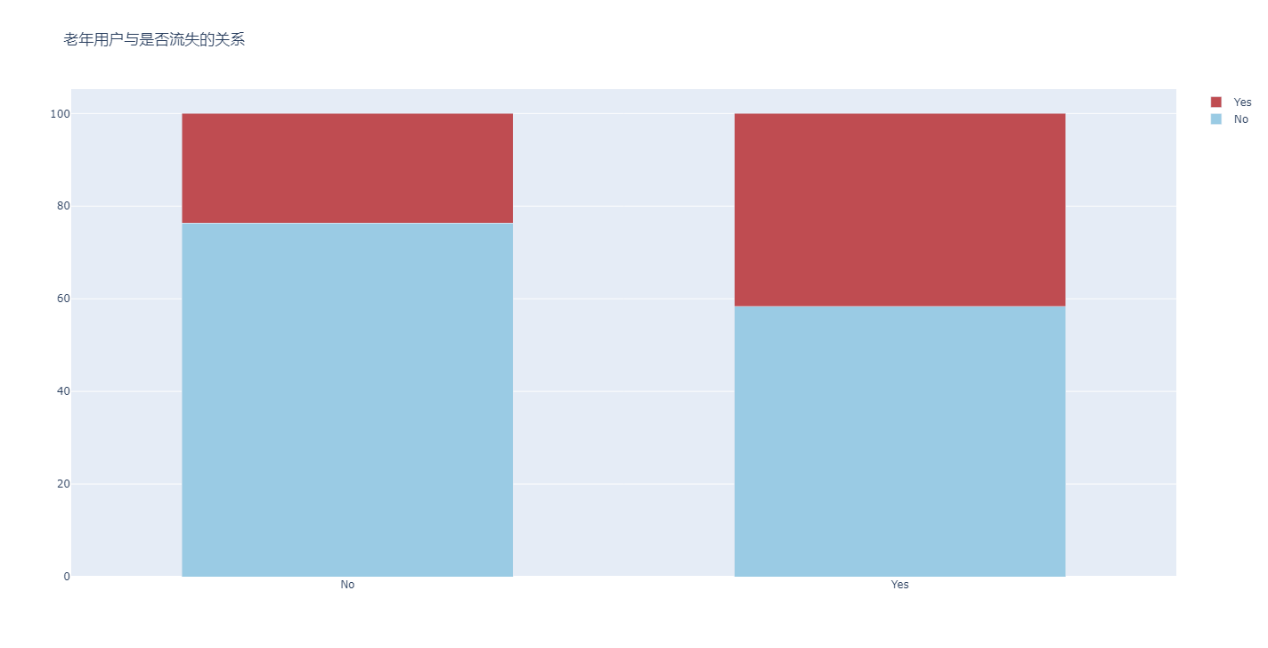
\includegraphics[width=\textwidth]{./img/t3.png}
\end{figure}
可以看出,老年用户流失比例更高,为41.68\%,比非老年用户高近两倍,此部分原因有待进一步探讨。
\begin{figure}[H]
	\centering
	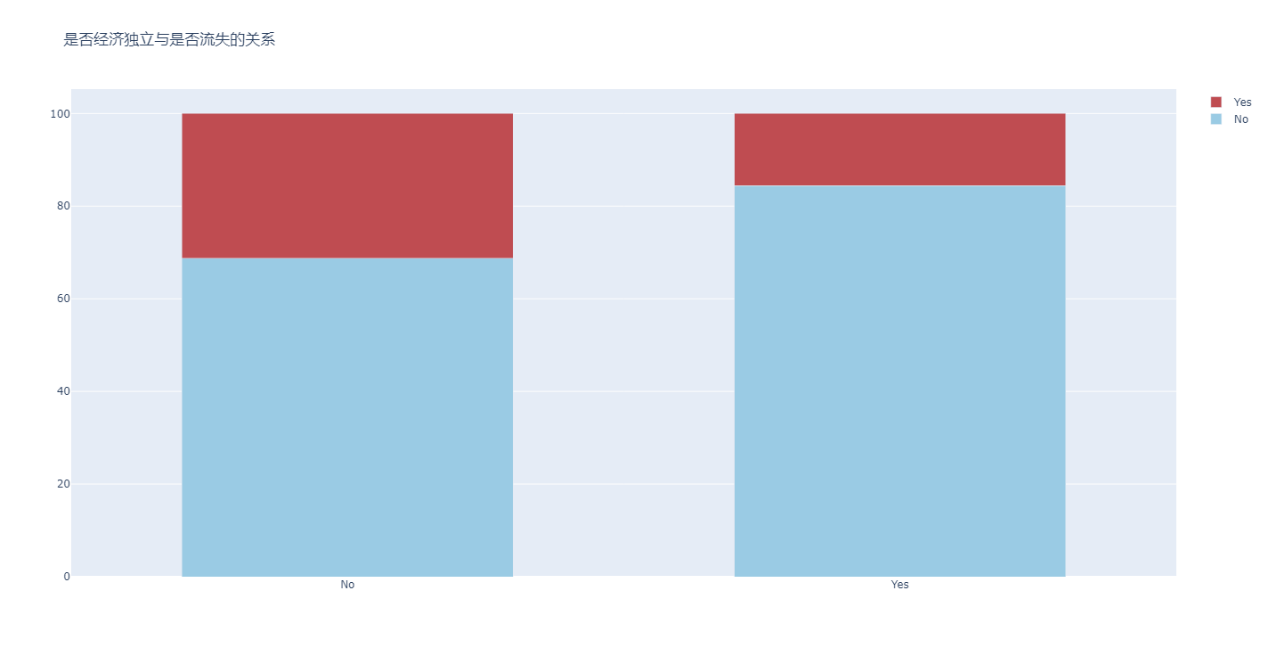
\includegraphics[width=\textwidth]{./img/t4.png}
\end{figure}
从经济独立情况来看,经济未独立的用户流失率要远远高于经济独立的用户。
\begin{figure}[H]
	\centering
	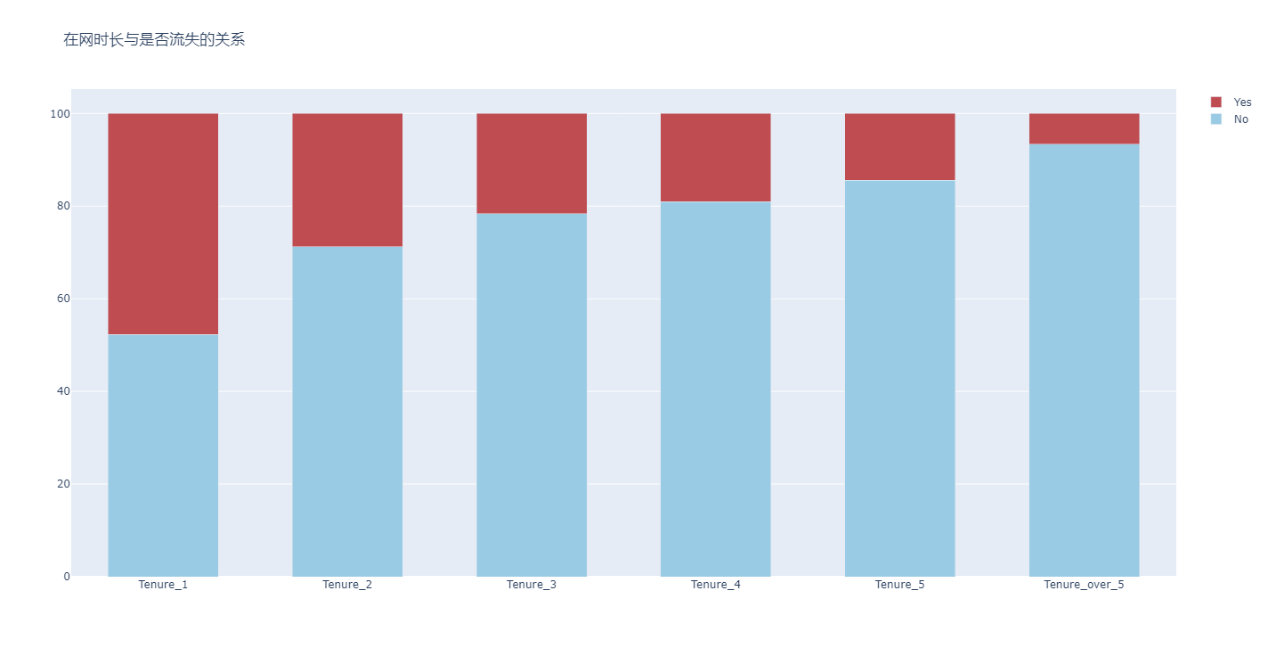
\includegraphics[width=\textwidth]{./img/t5.png}
\end{figure}
可以看出,用户的在网时长越长,表示用户的忠诚度越高,其流失的概率越低;新用户在1年内的流失率显著高于整体流失率,为47.68\%。
\begin{figure}[H]
	\centering
	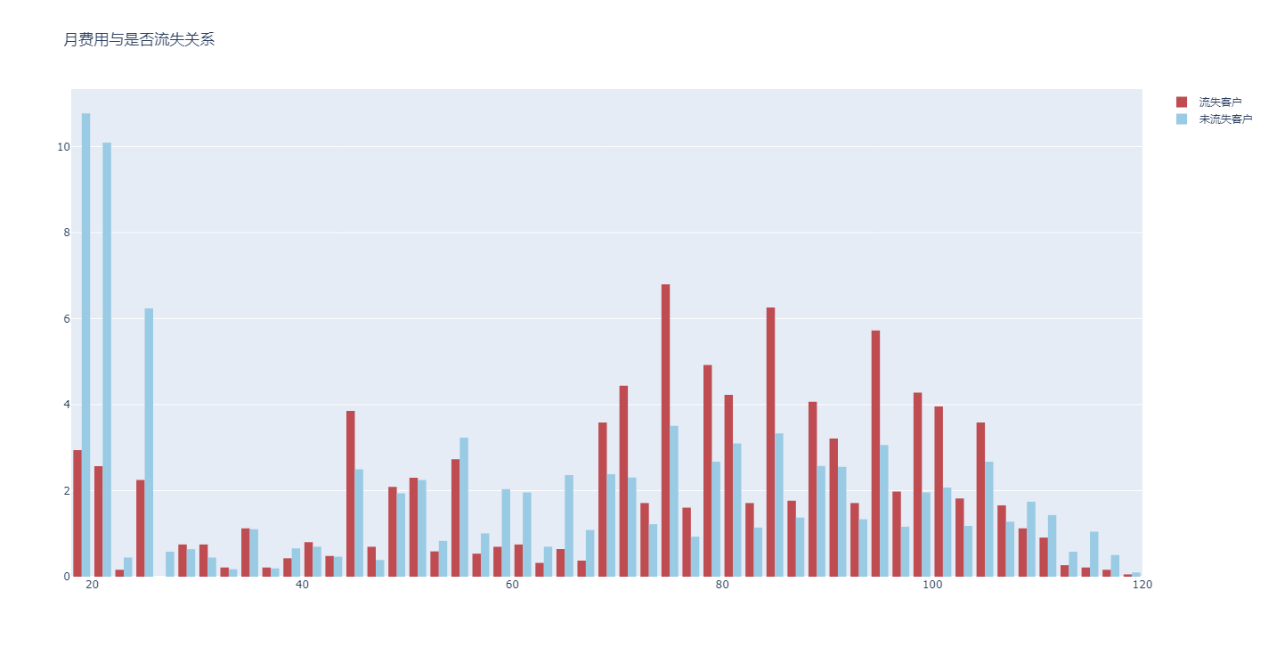
\includegraphics[width=\textwidth]{./img/t6.png}
\end{figure}
整体来看,随着月费用的增加,流失用户的比例呈现高高低低的变化,月消费80-100元的用户相对较高。
\begin{figure}[H]
	\centering
	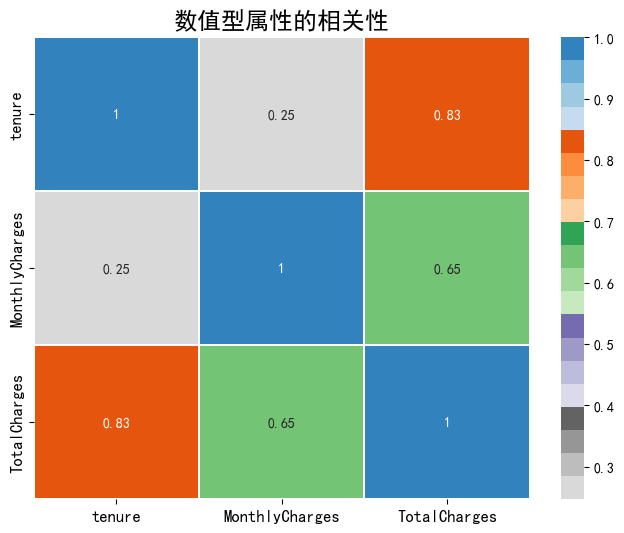
\includegraphics[width=\textwidth]{./img/t7.png}
\end{figure}
从相关性矩阵图可以看出,用户的往来期间(tenture)和总费用(TotalCharge)呈现高度相关,往来期间越长,则总费用越高。月消费和总消费呈现显著相关。

\section{模型构建}

\subsection{建立模型评估的框架}

\paragraph{k折交叉验证评估框架}

\begin{figure}[H]
	\centering
	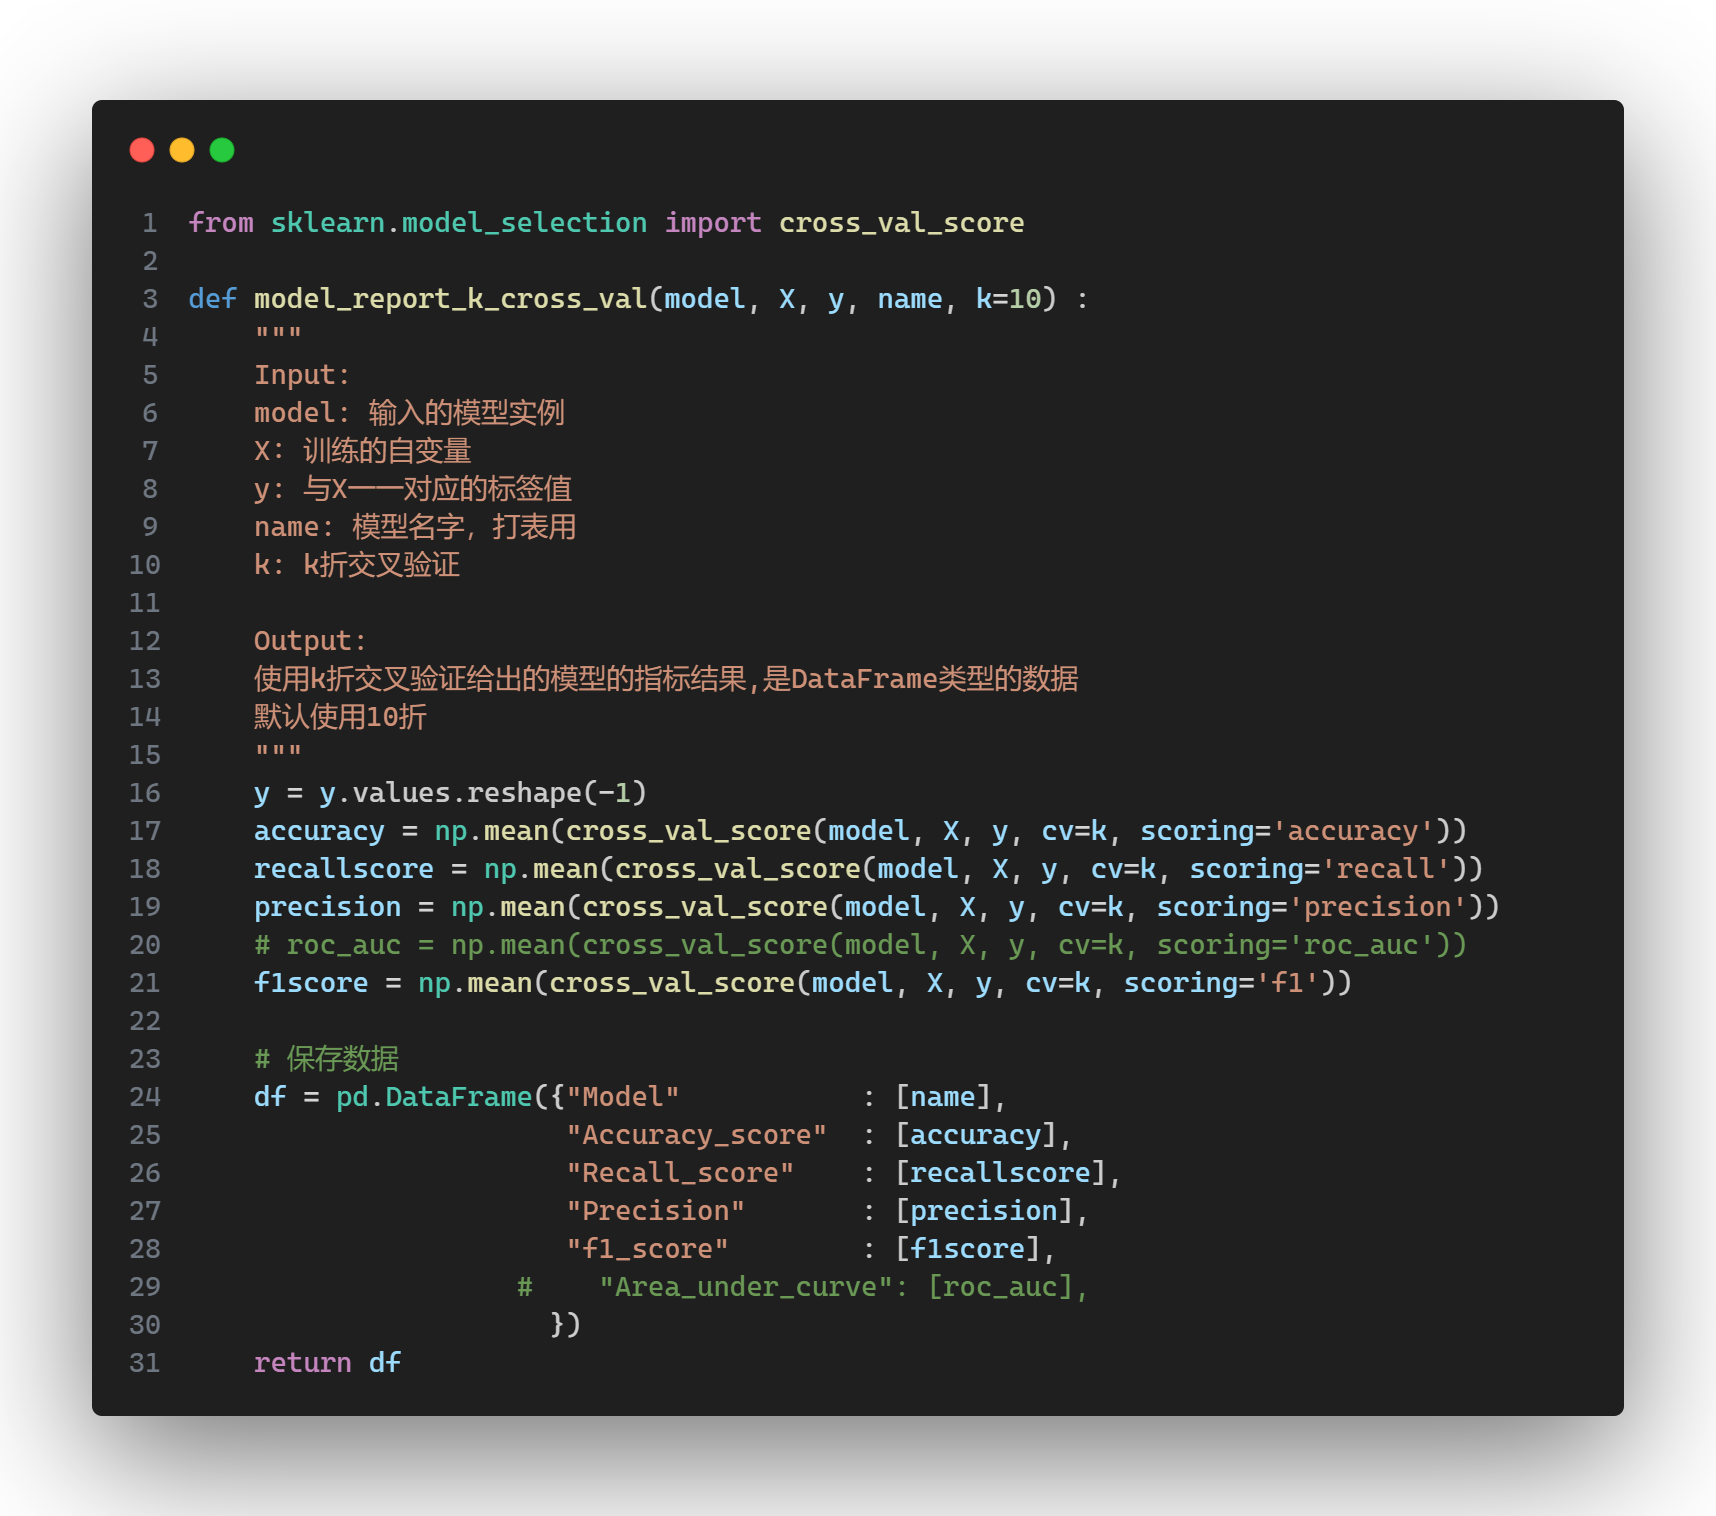
\includegraphics[width=\textwidth]{./img/k-cross-temple.png}
\end{figure}

这个框架接受一个输入的模型、数据、标签、模型名称、k值,给出k折交叉验证的评估指标结果,之后的所有模型评估都是用这个框架给出结果从而保证衡量的一致性和公平性。
由于我们直接调用了sklearn库中的cross\_val\_score函数,这个函数接受数据和标签的评估自然包含了测试集和训练集的划分方案,因此我们不需要进行手动的数据划分模块。


\subsection{模型定义和声明}

这里定义了一些基础的模型,待后续模型评估实验使用。
\begin{figure}[H]
	\centering
	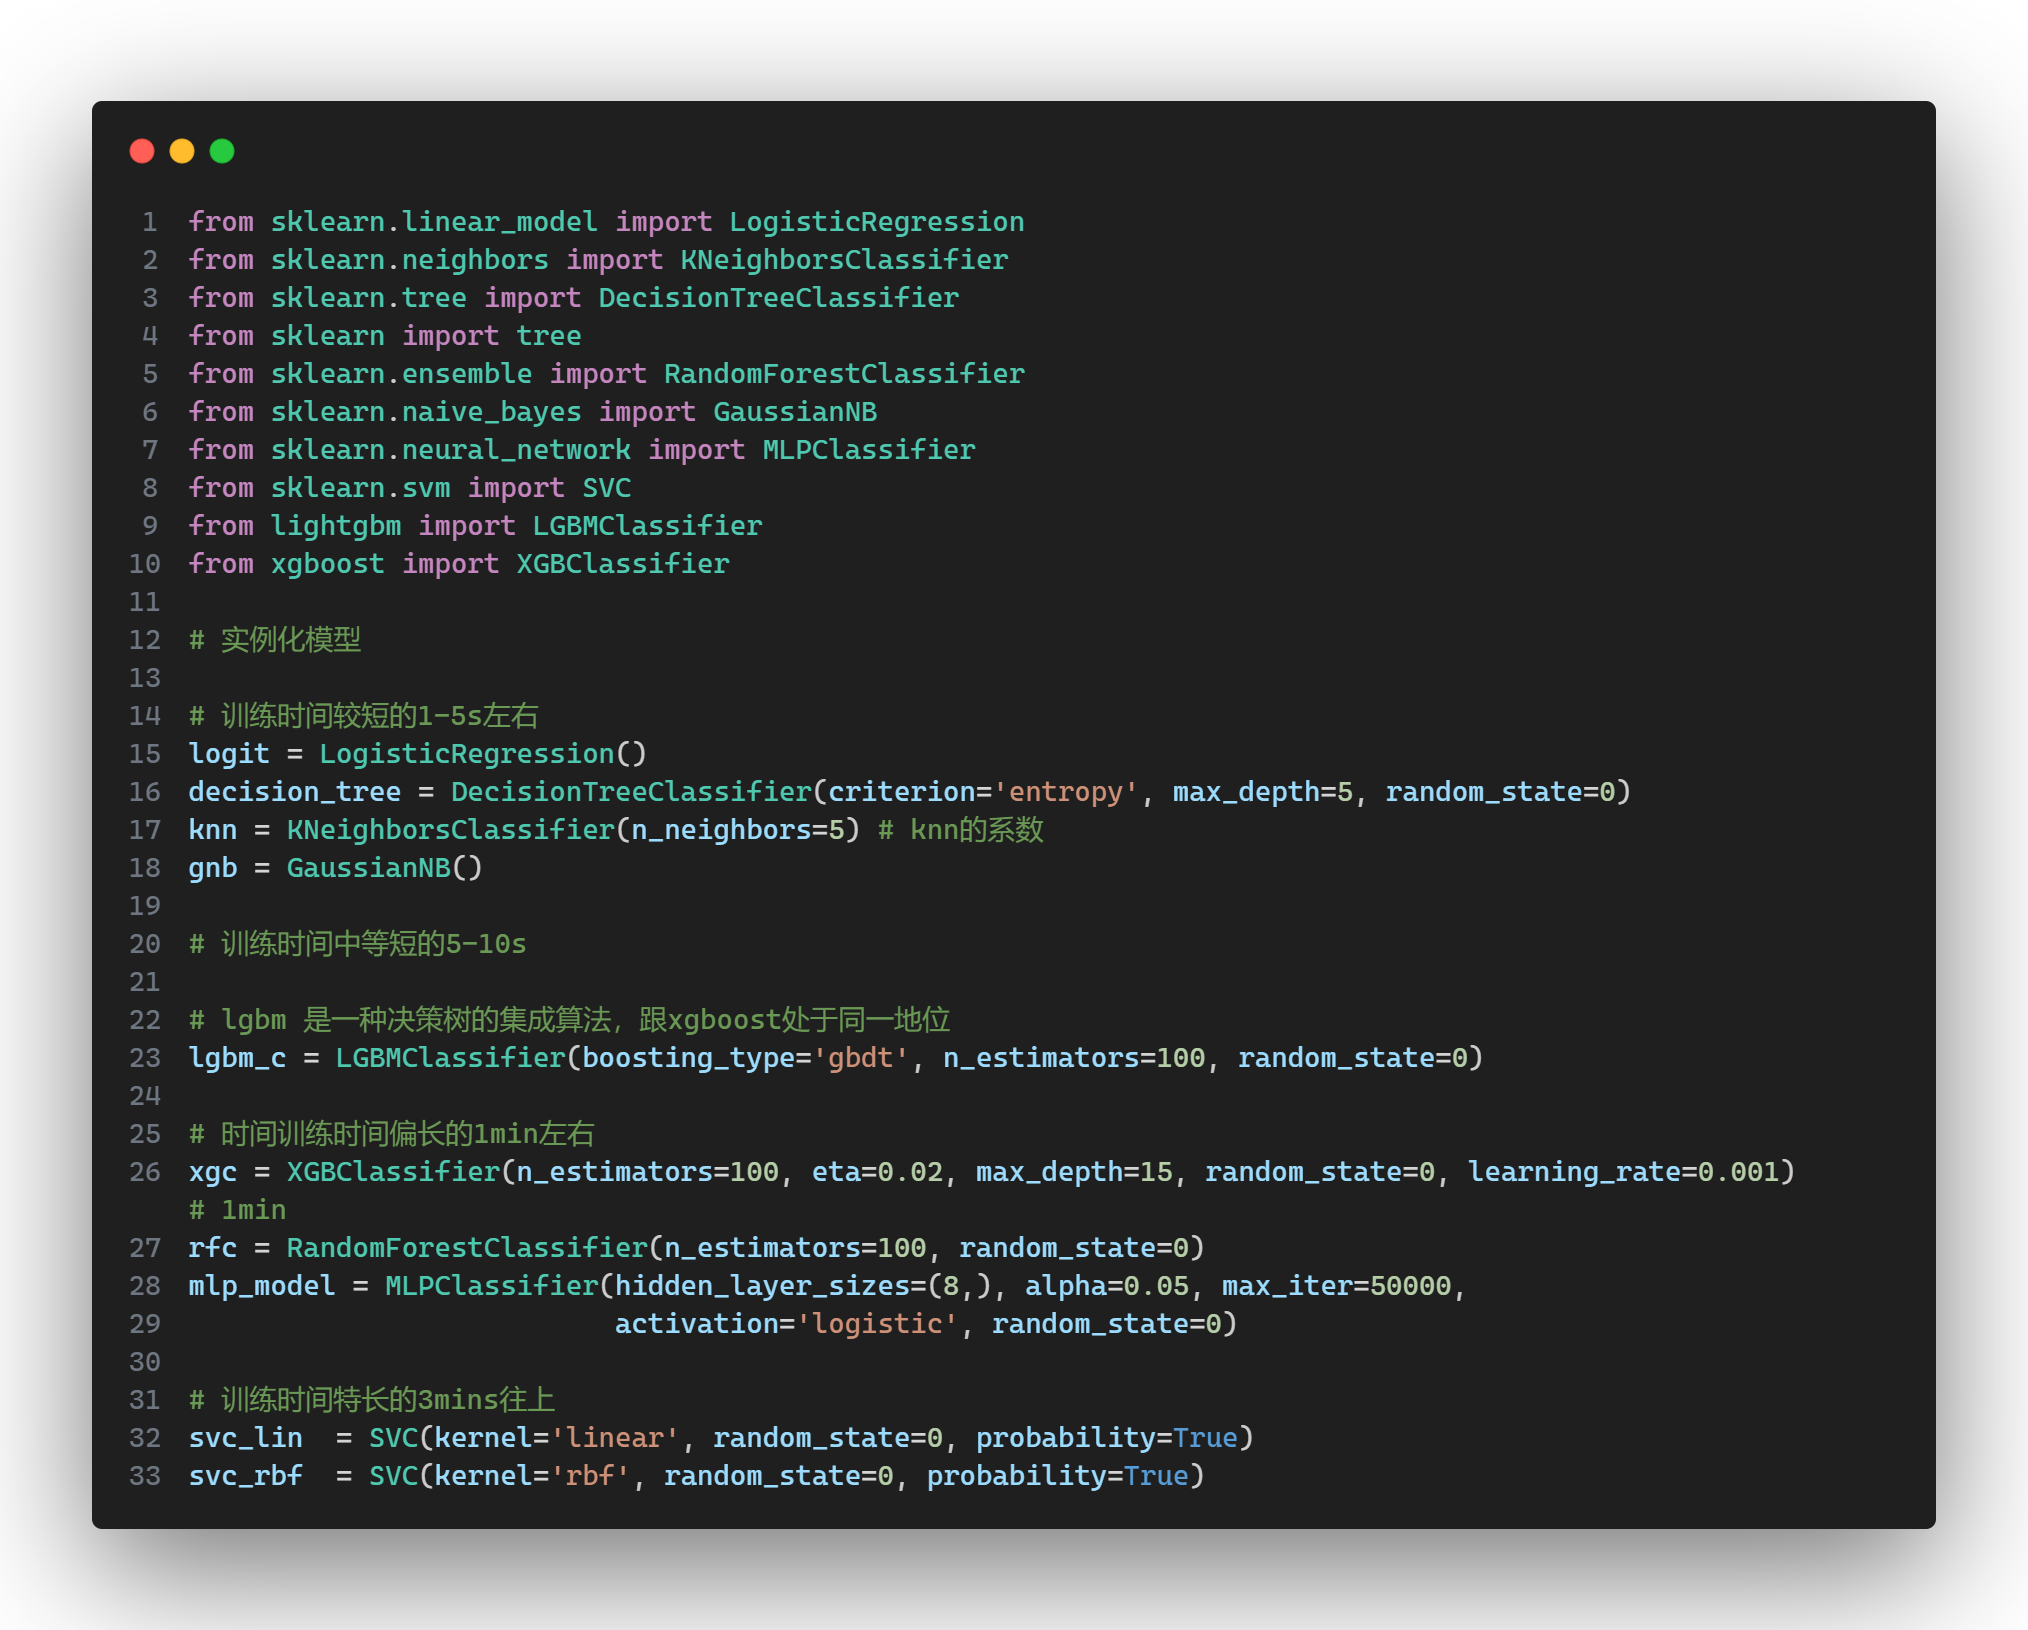
\includegraphics[width=\textwidth]{./img/models.png}
\end{figure}

\section{模型评估}
\subsection{对比不同数据压缩和变化在同一个模型上的效果}
为了查看各种数据降维的效果以及数据上采样后的效果,我们进行了如下实验的设计,写了一个函数,他接受一个模型,会将所有类型的预处理数据和原始数据在这个模型上跑一遍10折交叉验证
\begin{figure}[H]
	\centering
	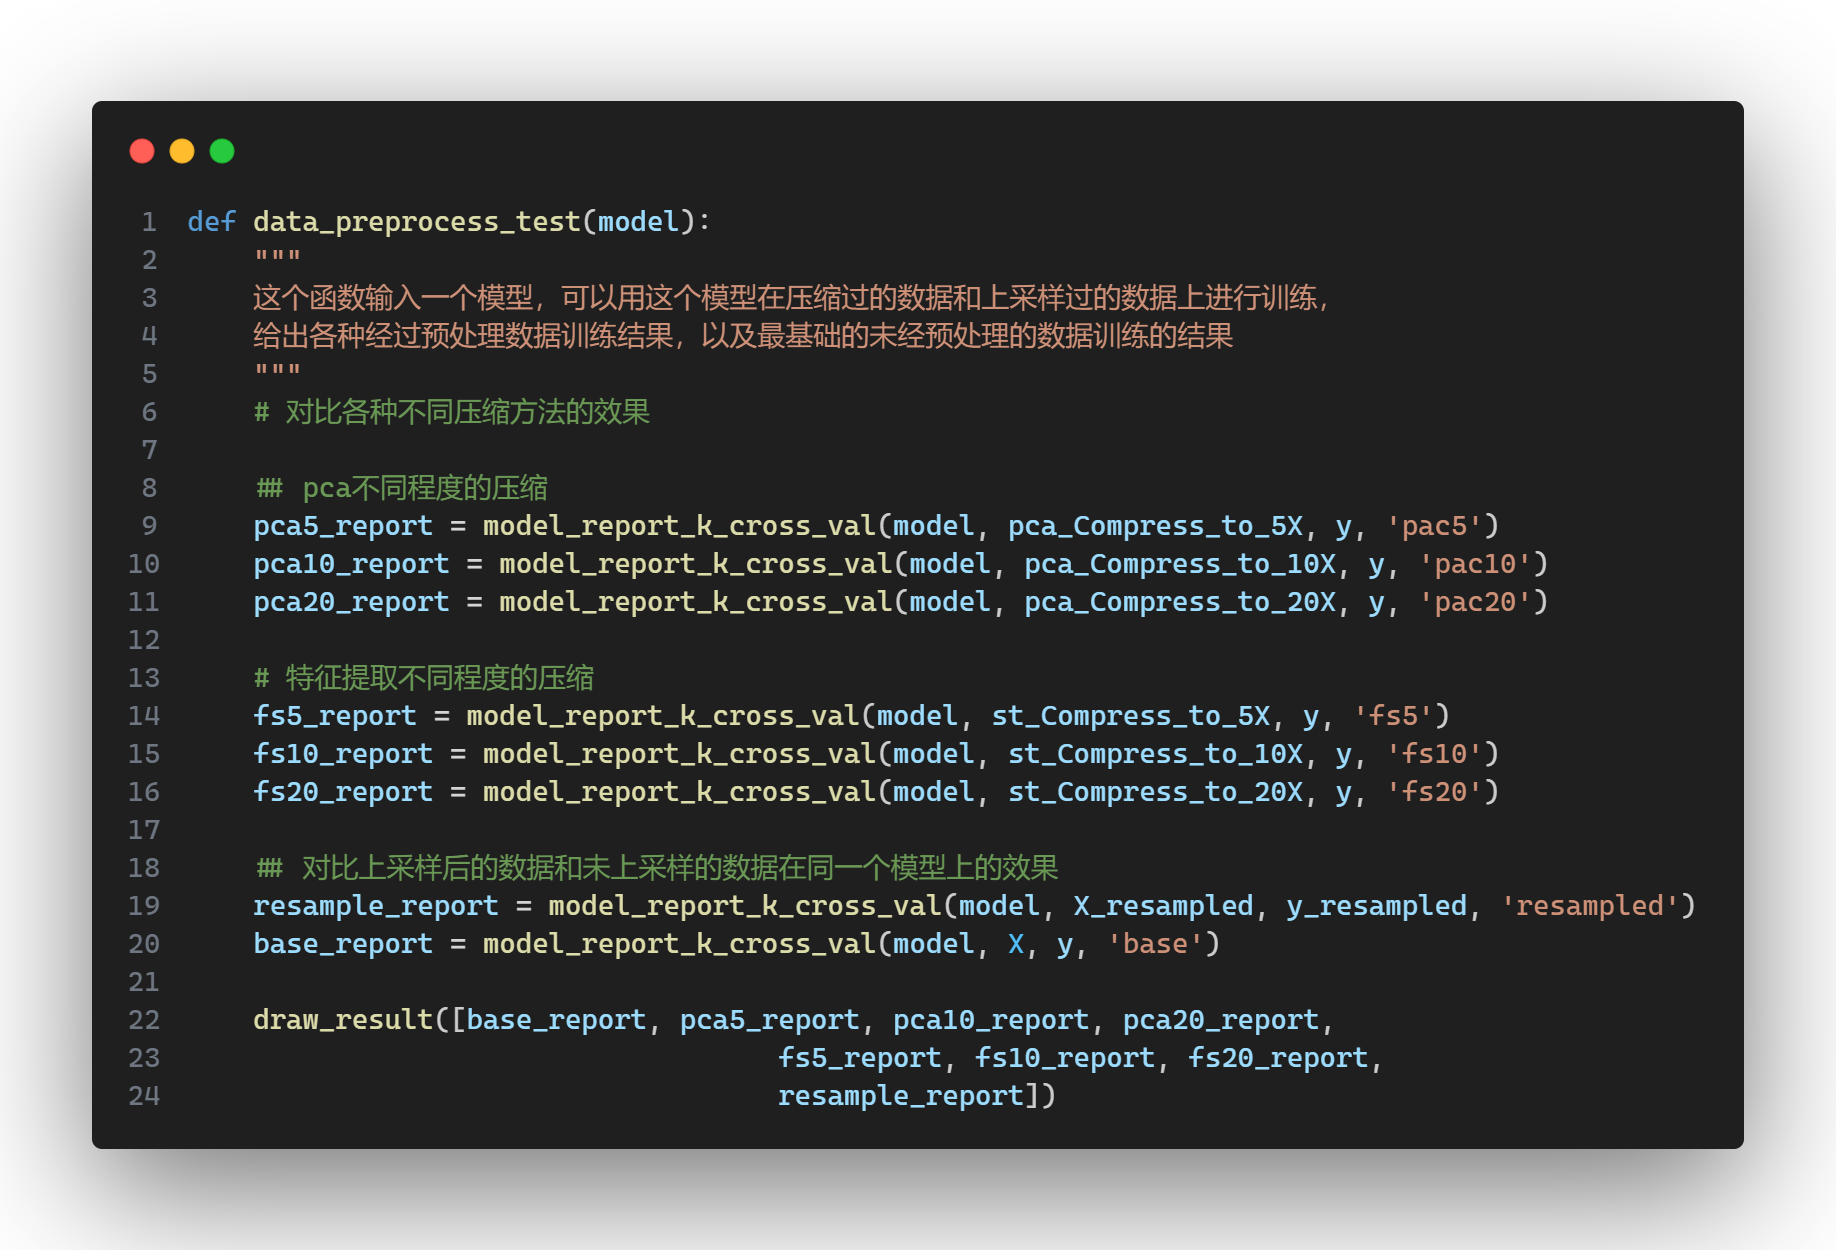
\includegraphics[width=\textwidth]{./img/data_prepocess_test.png}
\end{figure}


\begin{figure}[H]
	\centering
	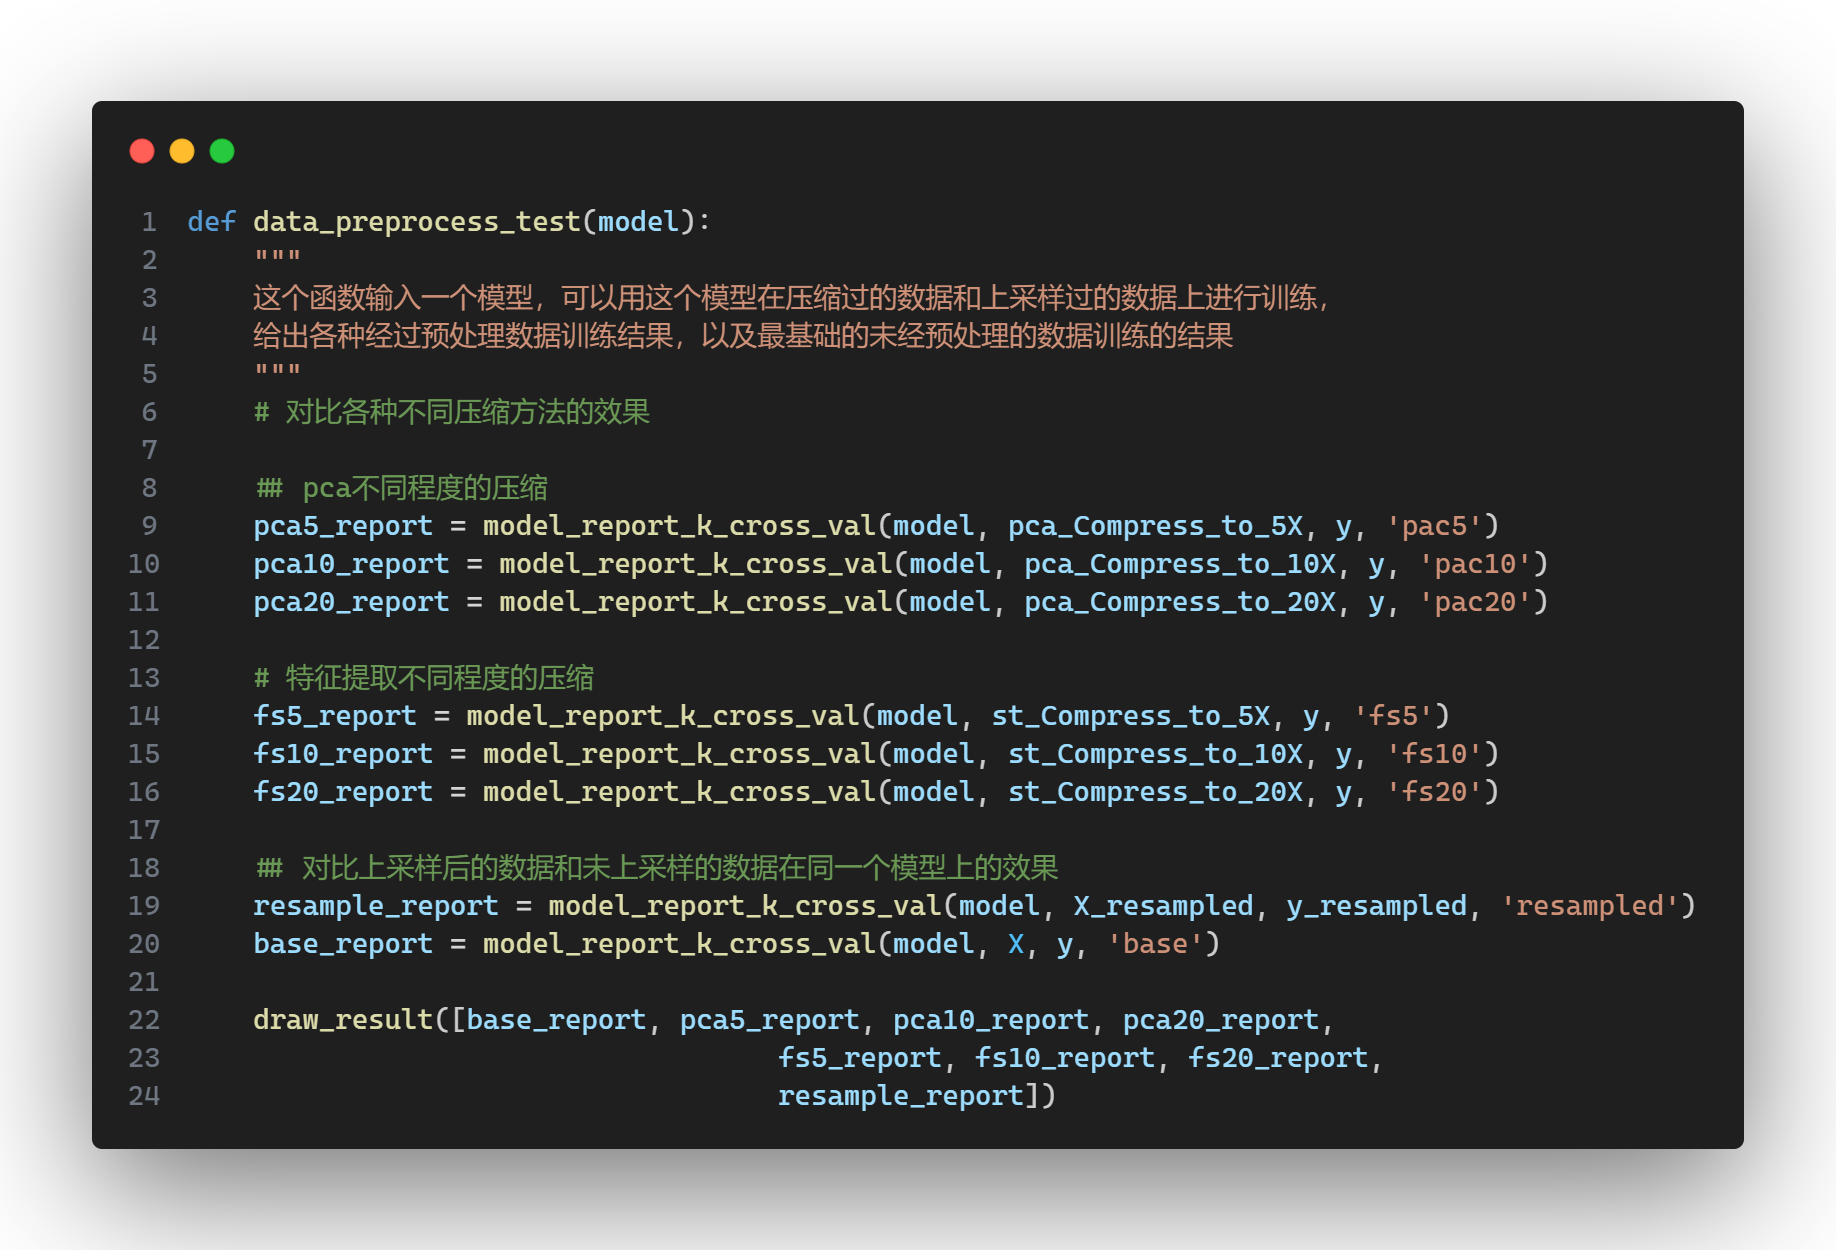
\includegraphics[width=\textwidth]{./img/data_prepocess_test.png}
\end{figure}

使用这个函数我跑了三个速度较快的模型进行对比,朴素贝叶斯分类器,逻辑回归,决策树

实验结果如下
\begin{figure}[H]
	\centering
	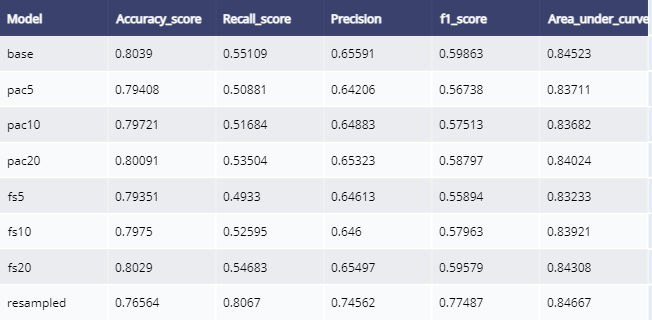
\includegraphics[width=\textwidth]{./img/logit_pre.png}
\end{figure}

\begin{figure}[H]
	\centering
	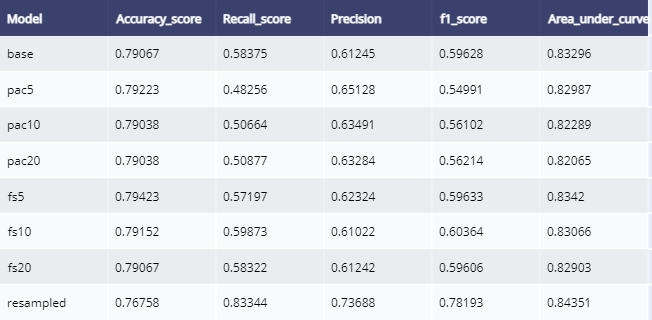
\includegraphics[width=\textwidth]{./img/dt_pre.png}
\end{figure}

\begin{figure}[H]
	\centering
	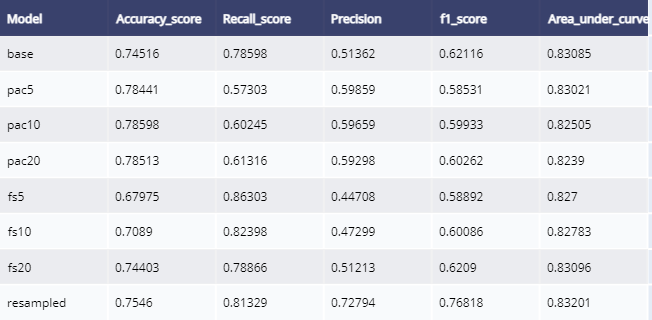
\includegraphics[width=\textwidth]{./img/gnb_pre.png}
\end{figure}

通过上述实验结果我们可以看出来,通过上采样对于模型的效果提升最好,在所有的指标上有提升;同时我们也发现,两种数据降维的压缩方式对于模型反而有了负面效果,至少在贝叶斯分类器上是这样的效果,或许是由于朴素贝叶斯分类器对于冗余数据的抗干扰性较强,或是这些属性本身的相关程度就不大,因此自变量被减少之后,导致了信息量的真实损失,而不是解除了维度诅咒,因此导致效果变差。
因此得出结论,指导我在之后的操作过程中直接使用上采样的平衡数据,不要采用降维方法应该会得到更好的效果,因此在后续的实验中我们直接采用重采样后的平衡数据做模型训练。

\subsection{使用上采样的数据将各种模型都跑一遍10折交叉验证对比效果}
代码如下:
\begin{figure}[H]
	\centering
	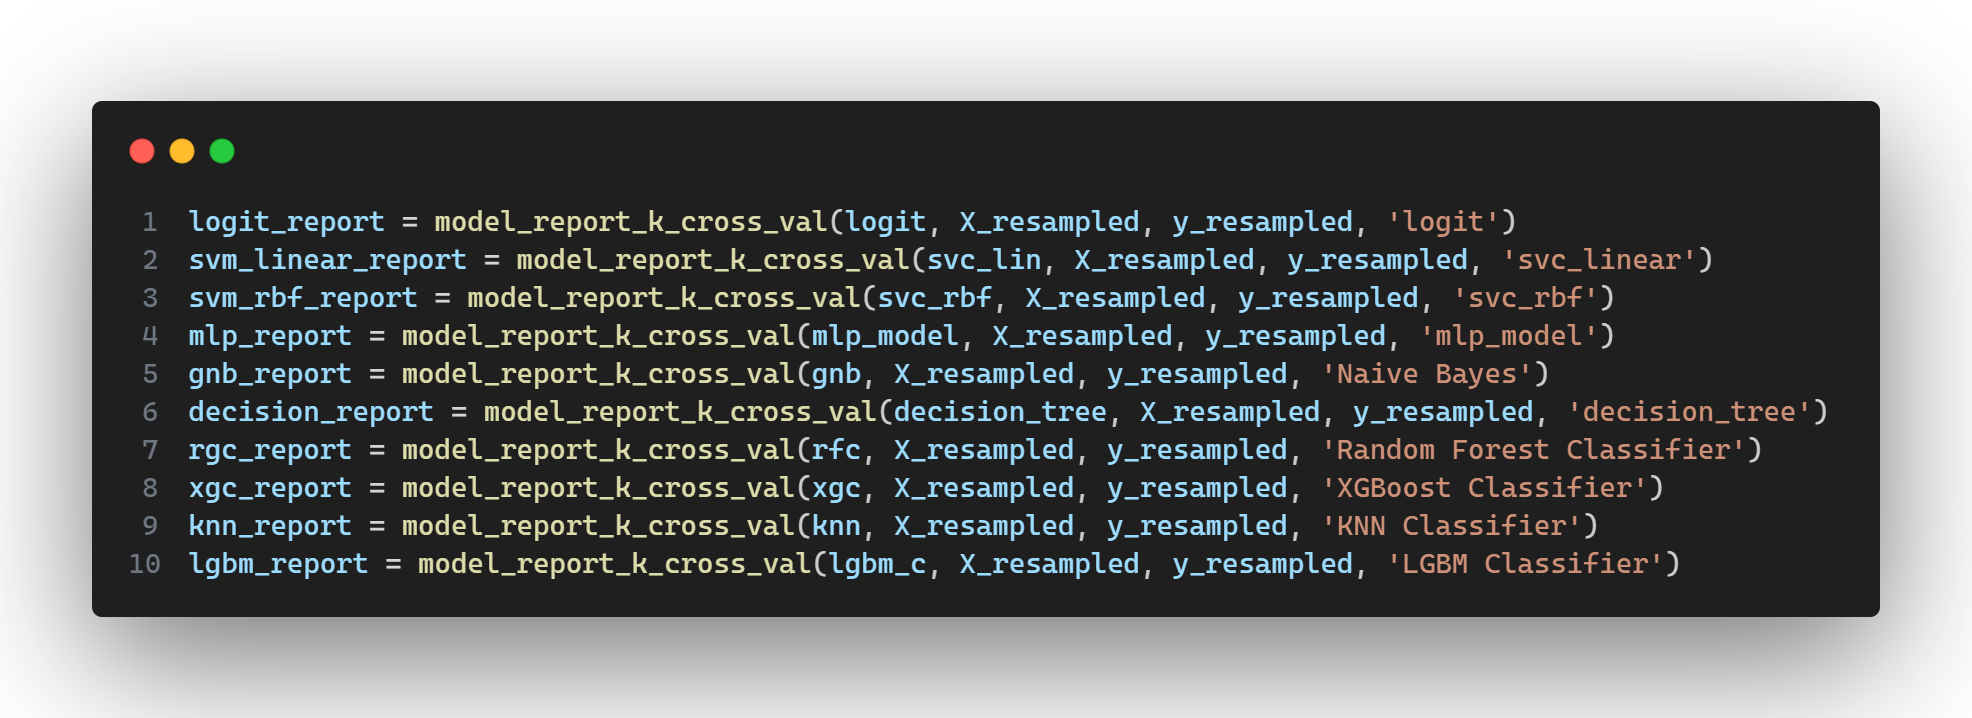
\includegraphics[width=\textwidth]{./img/test_all_models.png}
\end{figure}

结果如下
\begin{figure}[H]
	\centering
	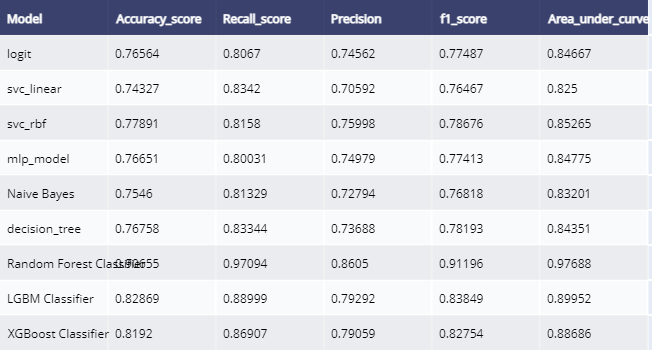
\includegraphics[width=\textwidth]{./img/all_models_res.png}
\end{figure}

从上述的结果我们可以看出来使用了集成思想的后面三个模型的所有指标都显著高于前面的那些单一模型,
尤其是随机森林的效果最好,召回率和auc面积都达到了97\%以上的精确率,
可以说是非常高的水平了,改良的效果很好,由于我们使用的是10折交叉验证,
因此这个结果具有可信度,不是随机导致的某次结果很好产生的效果。

而下面是老师提供的baseline方法的效果:

\begin{figure}[H]
	\centering
	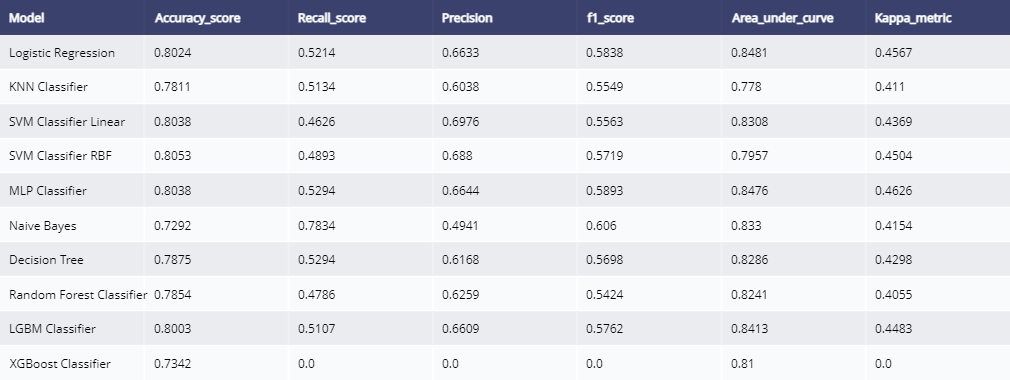
\includegraphics[width=\textwidth]{./img/baseline_result.png}
\end{figure}

和未经数据上采样的各项指标对比,我们会发现各个模型要么有很大的提升,
要么会有很小的提升,但是都没有出现负面的效果,而其中提升最显著的就是决策树相关的四种算法,
说明决策树对于数据不平衡较为敏感,且在数据平衡后,能产生非常好的效果。

\subsection{手动实现集成的过程}

我们知道决策树是一种不稳定的算法,虽然库中已经提供了他的很多集成算法模型, 但是为了手动体验这个过程,我打算自己实现一遍集成的算法看看能否提高性能,具体来说,
我采用的bagging方法,实现了一个满足sklearn库模型接口的类my\_bagging\_decision\_tree,
这个自己实现的模型类中使用了bagging的方式集成了多个决策树模型, 使用最大数投票原则给出了最终的分类结果,同时,实现了10折交叉验证的分数计算接口,
实现了和打框架的特匹配和统一,可以直接调用cross\_val\_score函数进行交叉验证,给出模型效果指标。

具体的函数如下:
\begin{figure}[H]
	\centering
	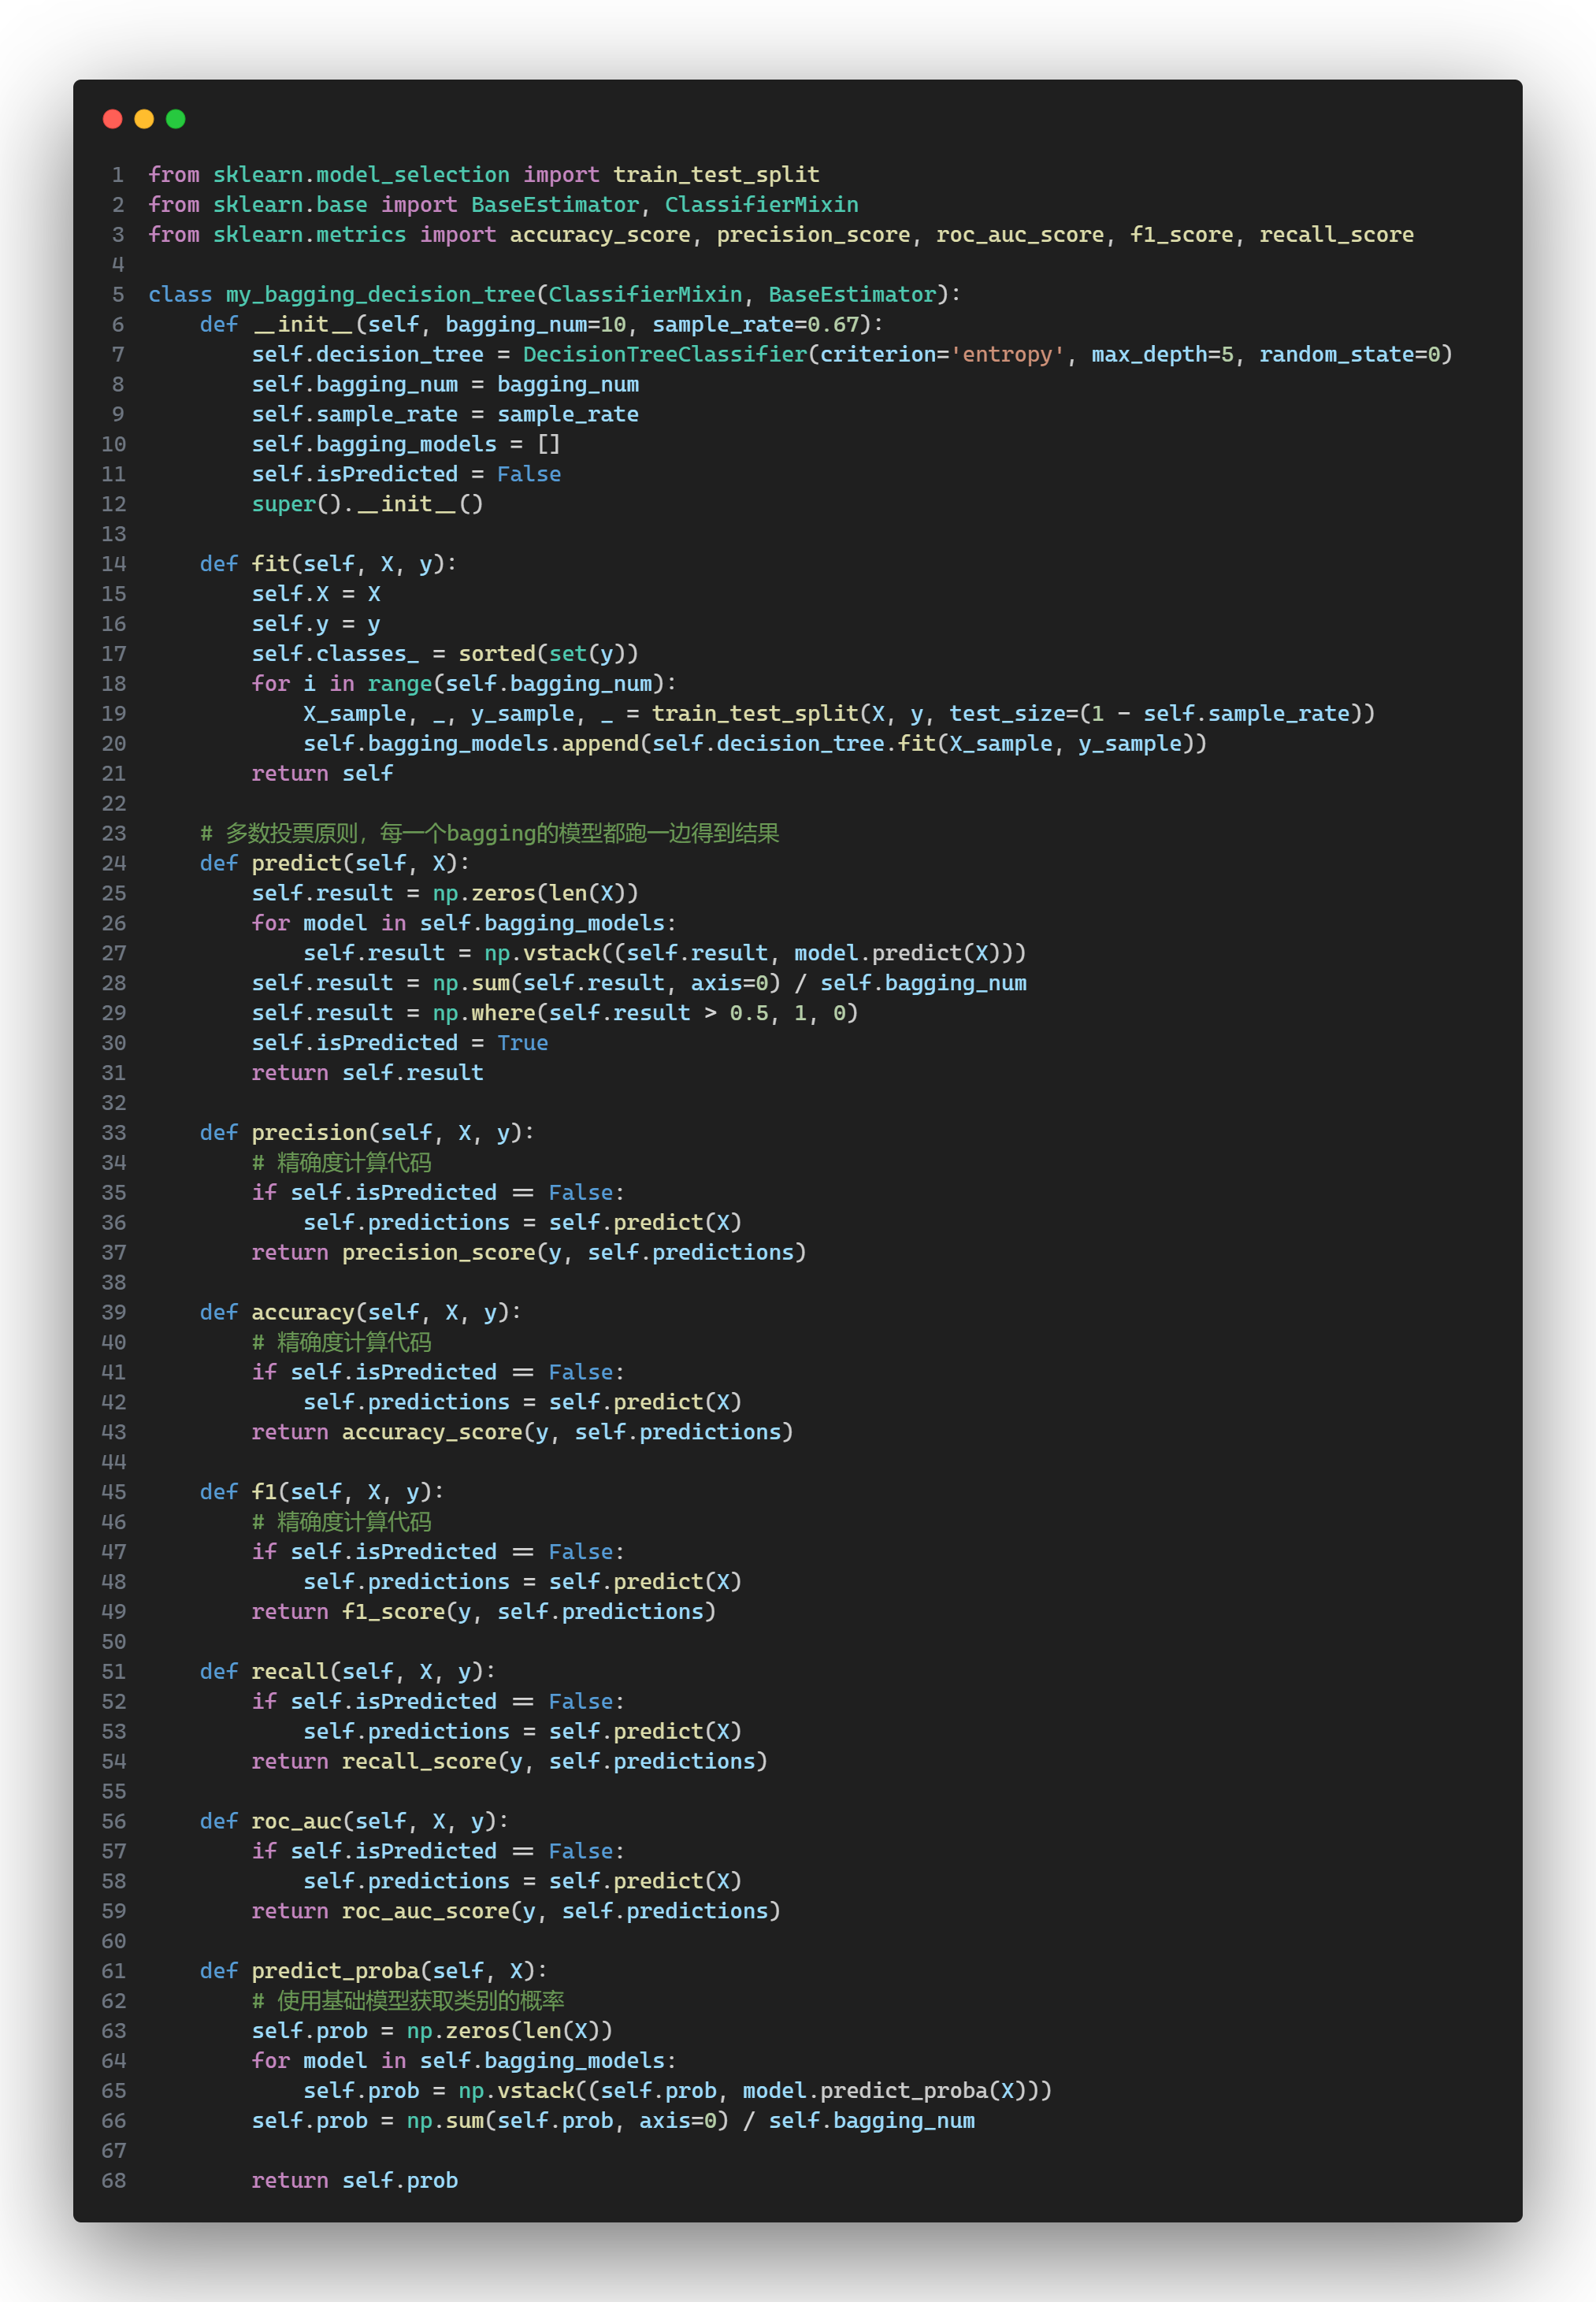
\includegraphics[width=\textwidth]{./img/hand_bagging.png}
\end{figure}

\subsection{集成不同类别的分类器}

\begin{figure}[H]
	\centering
	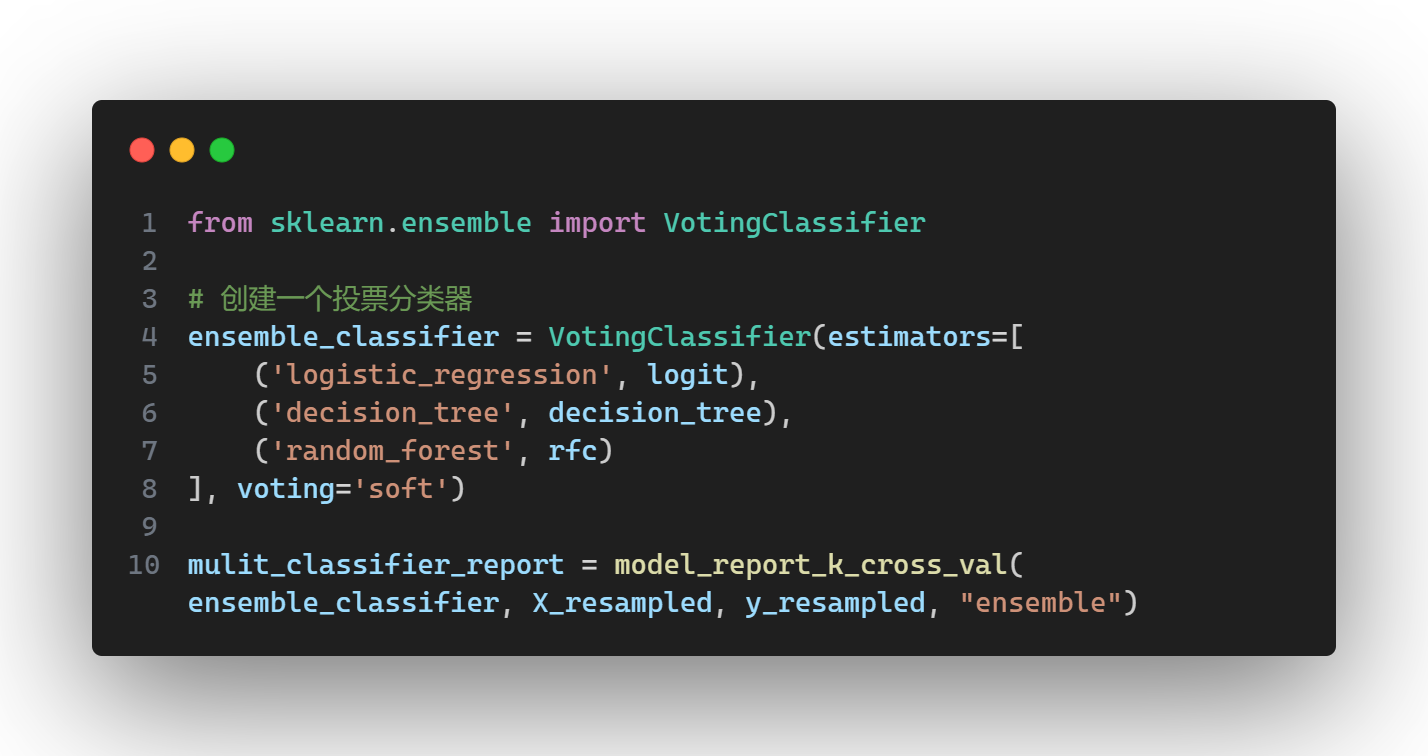
\includegraphics[width=\textwidth]{./img/mult_voting.png}
\end{figure}

结果如下
\begin{figure}[H]
	\centering
	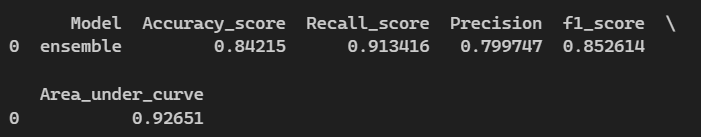
\includegraphics[width=\textwidth]{./img/voting_res.png}
\end{figure}

通过上面的实验,我们可以发现,如果集成的分类器有稳定的也有不稳定的,不稳定的分类器反而会将本来效果很好的稳定的分类器的性能给拉低,因此没有将弱分类器和强分类器结合的必要。

\subsection{决策树调参}

\begin{figure}[H]
	\centering
	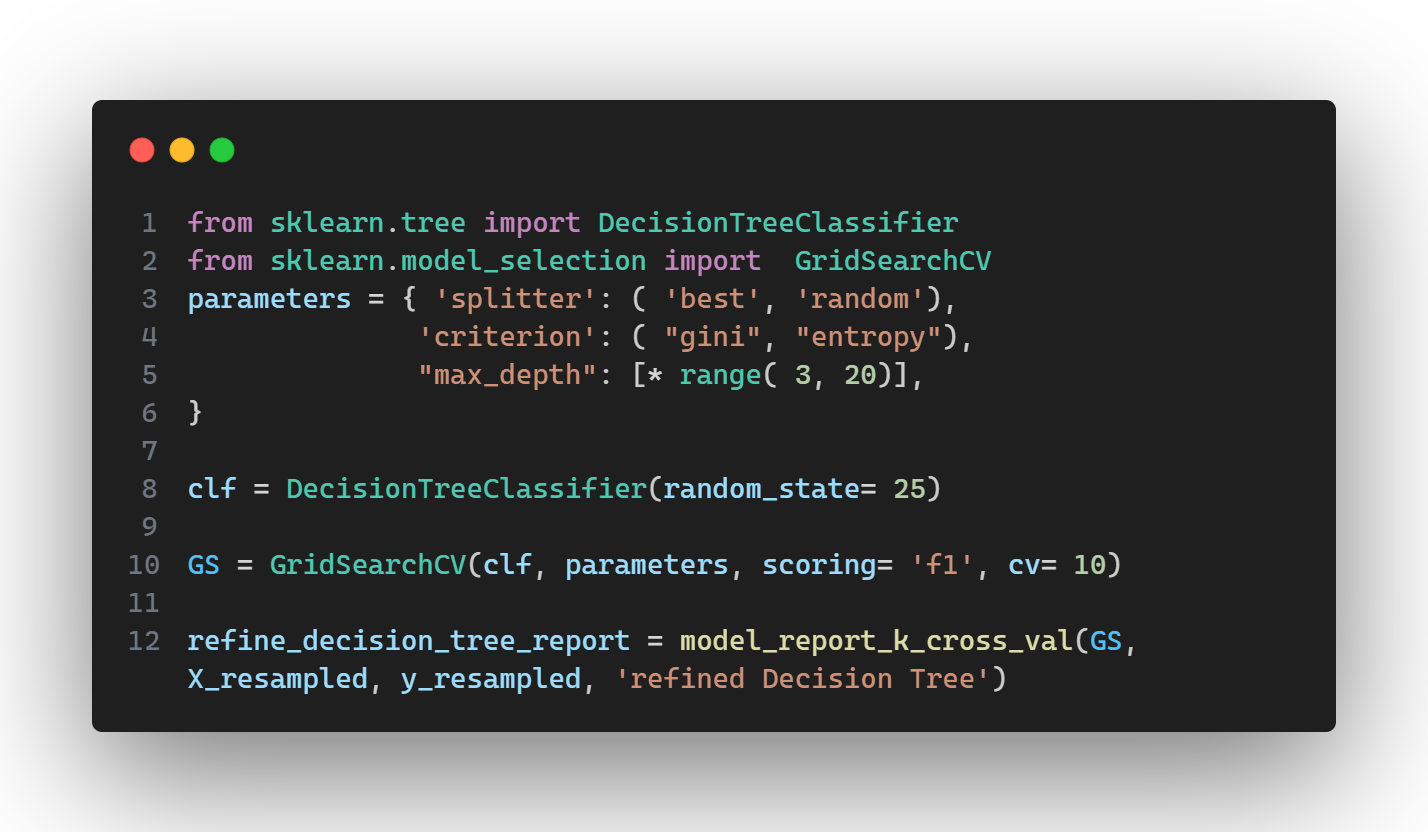
\includegraphics[width=\textwidth]{./img/refine_dt.png}
\end{figure}

决策树调参后的结果如下:

\begin{figure}[H]
	\centering
	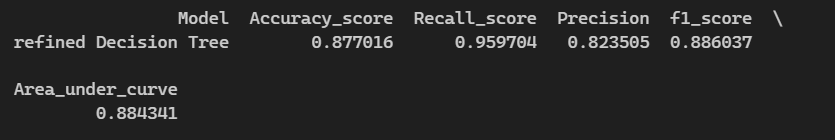
\includegraphics[width=\textwidth]{./img/refine_res.png}
\end{figure}

我们可以发现相较于不调参的决策树,这个调参后的效果要更好


\subsection{尝试自己实现一个MLP的模型}
这是数据加载器的定义部分
\begin{figure}[H]
	\centering
	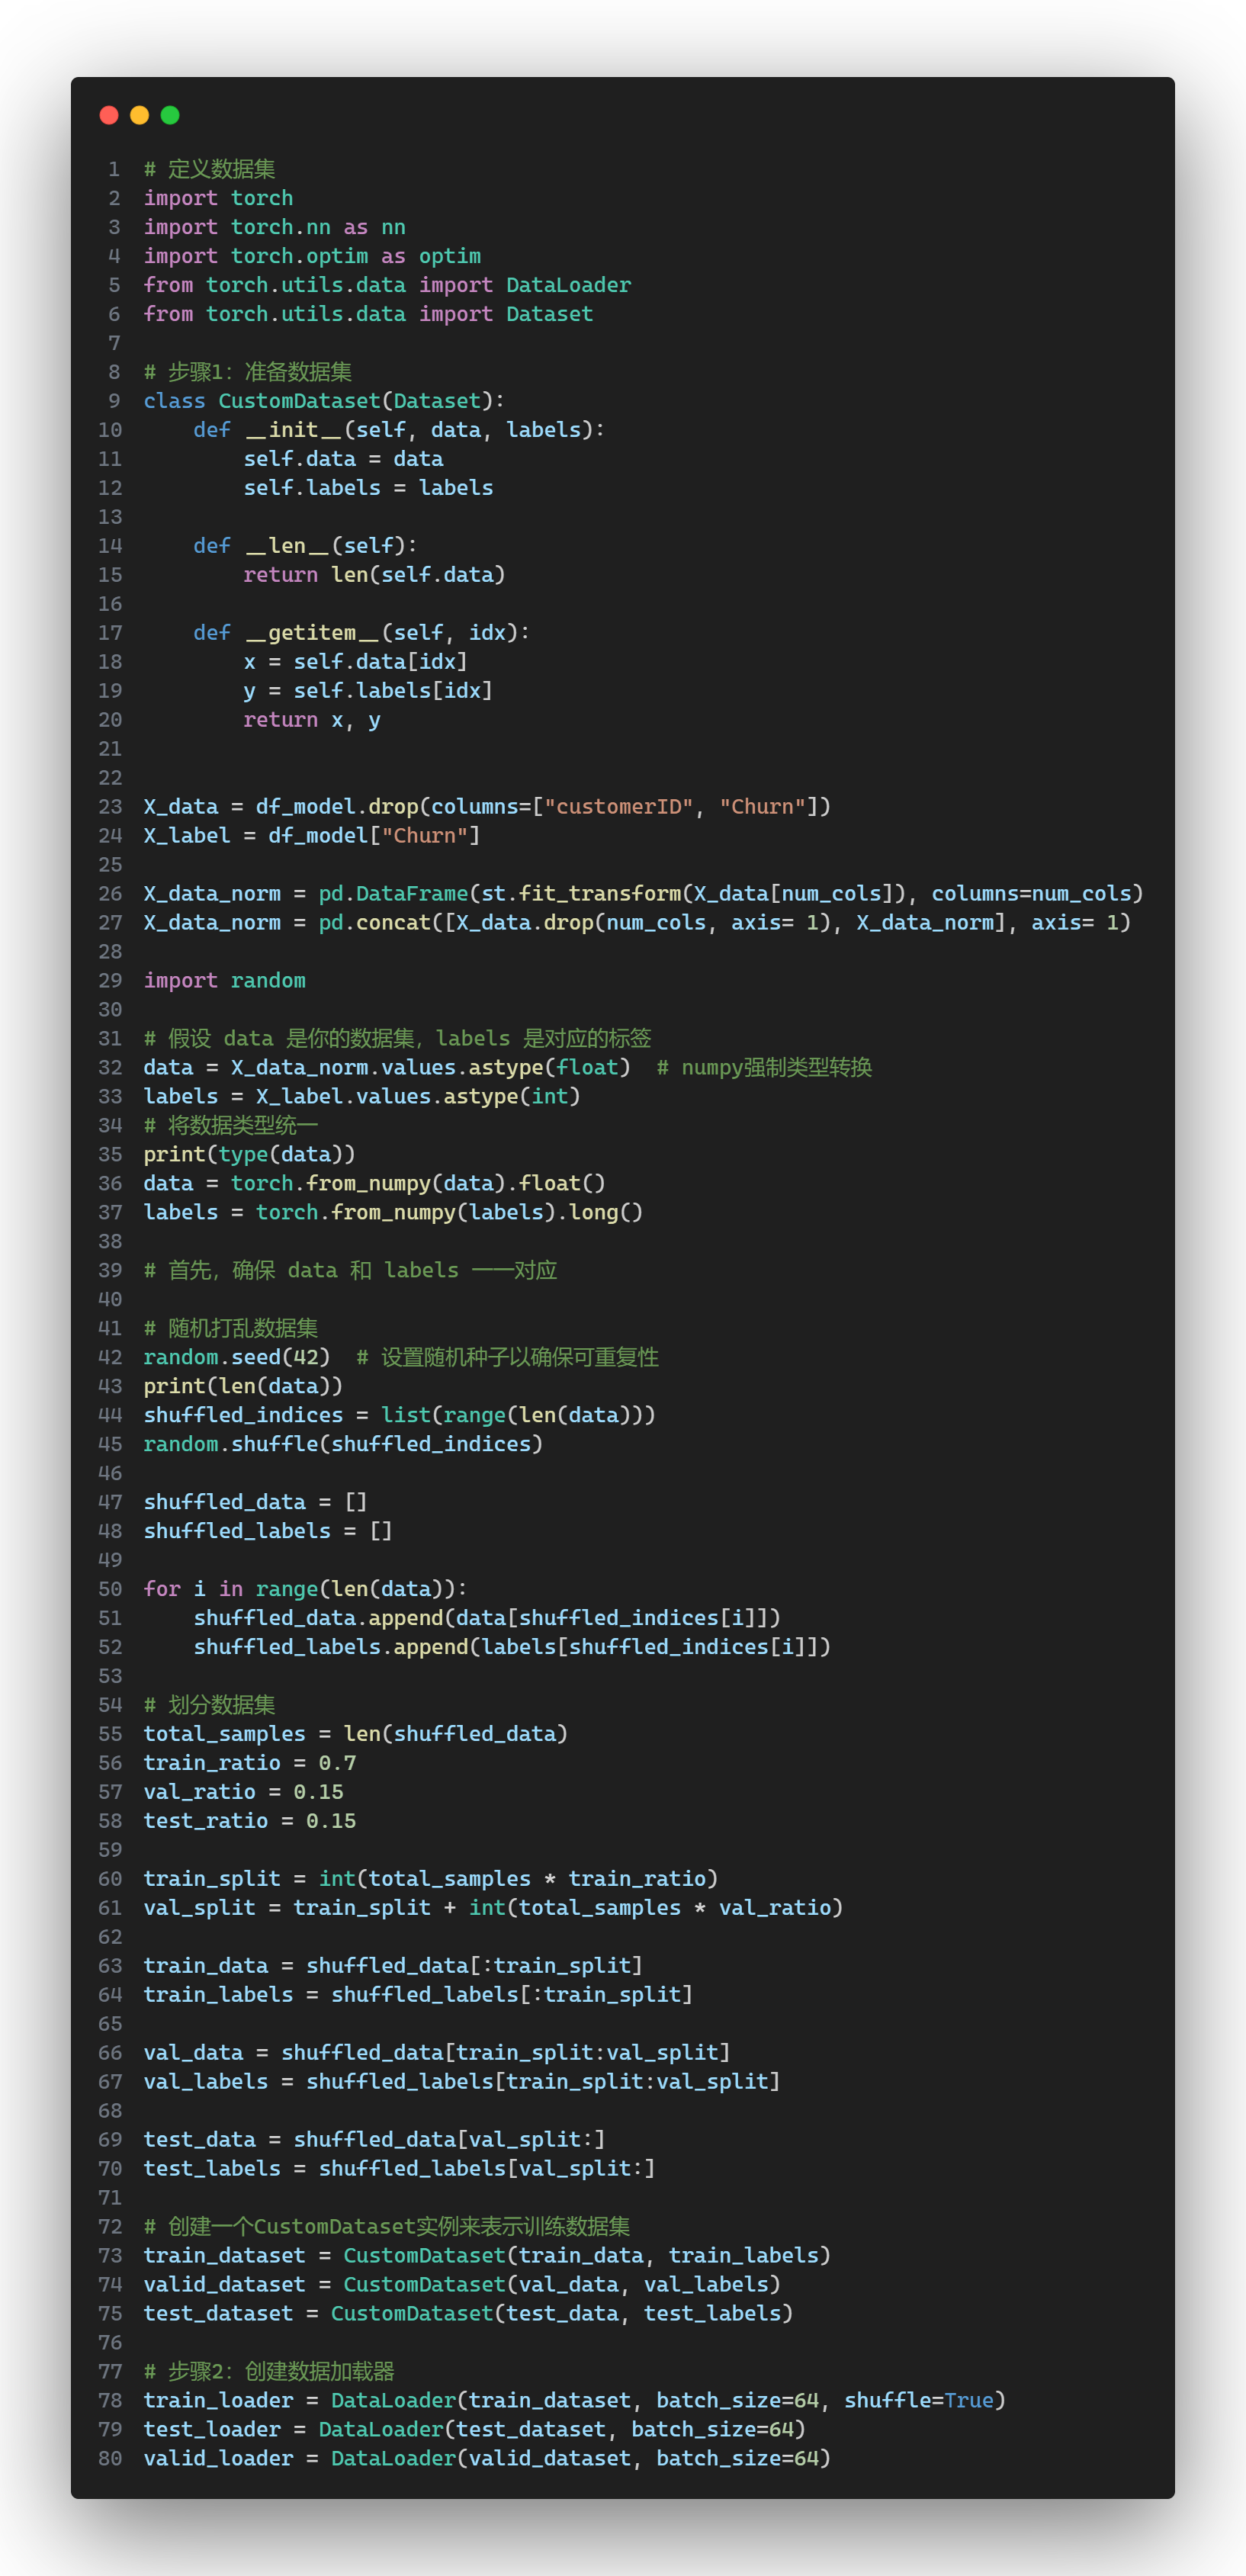
\includegraphics[width=\textwidth]{./img/mlp1.png}
\end{figure}

使用了如下定义的模型,输入层有32个神经元作为特征提取层,接下来的两层中间层神经元数量分别为100、2,计算损失函数时还有一个softmax层作为输出层,构造代码如下:
\begin{figure}[H]
	\centering
	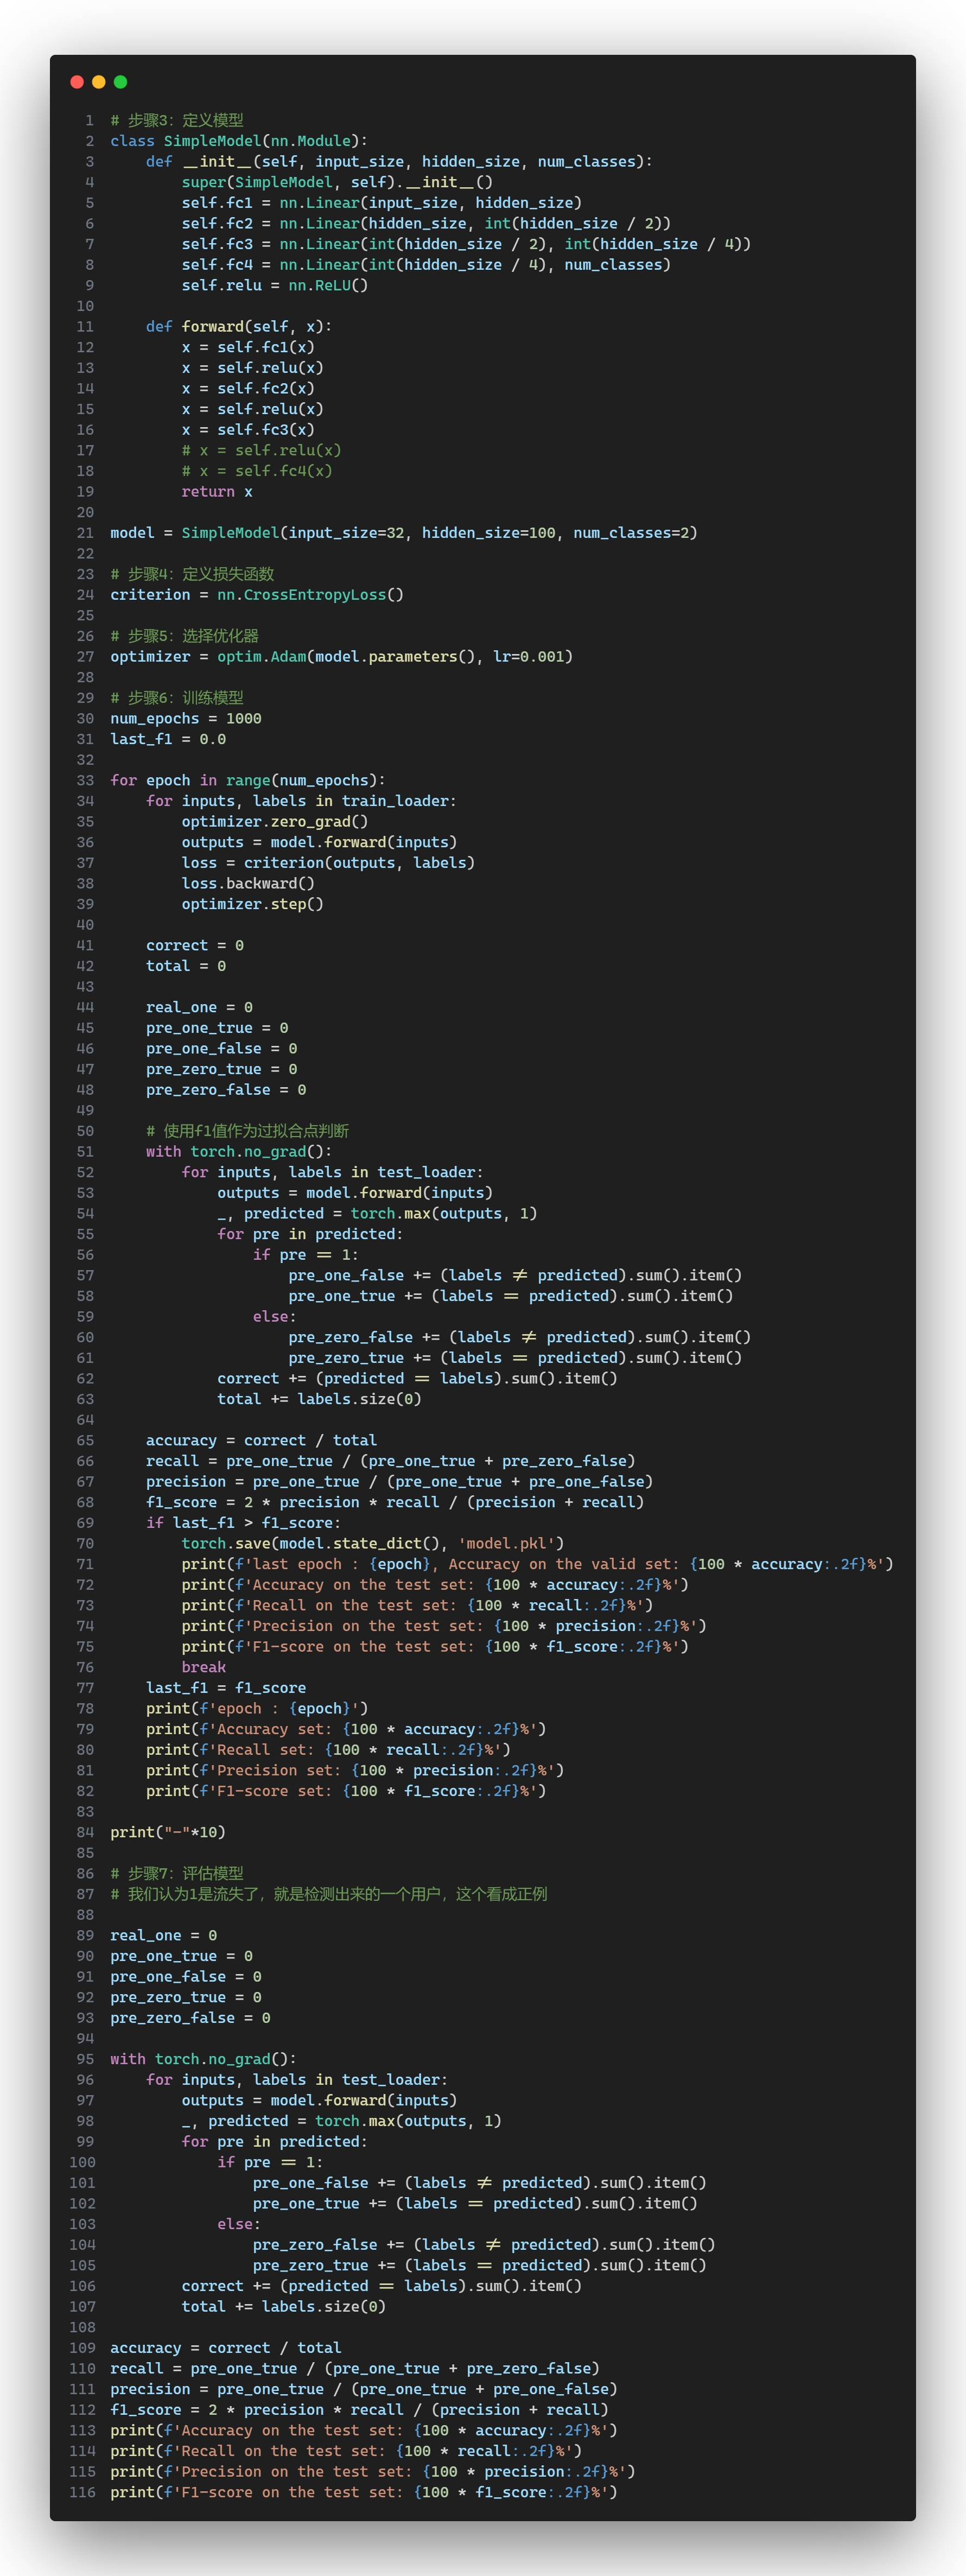
\includegraphics[width=\textwidth]{./img/mlp2.png}
\end{figure}



\begin{figure}[H]
	\centering
	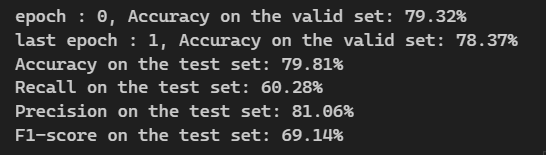
\includegraphics[width=\textwidth]{./img/my_mlp_res.png}
\end{figure}
虽然这个网络结构较为简单,层数也不多,但是给出的效果是和上述baseline中的最好的结果不相上下的。
虽然数据集的划分是不变的,但是每次我们训练出来的模型迭代到的最佳性能值都有所差别,这也反应出来了神经网络对函数的拟合是局部最优而不是全局最优,因此导致每次初始化的值不同,迭代的方式的随机性导致的最终得到的模型性能差异有所区别,但是在这个应用场景下,数据量也不是很大,我们可以通过多次尝试找到最大F1值作为最终最优的模型输出。
细致观察召回率、精确率和准确率这三个指标,我们还能发现如下规律:每次训练出来的模型,在测试集上给出的结果都是十分接近的
80\%左右,没有很大的差异,而主要的变化在于精确率和召回率,如果我们再做横向对比,会发现其他几个baseline中的基本模型给
出的准确率也都是在80\%左右,这是一个值得探索的问题,而深度学习对于f1值的提升主要来自于精确率和召回率的提升召回率相比
于除贝叶斯模型的其他所有模型有10\%的提升,精确率则超过了所有的baseline中的模型10\%-30\%,因此综合表现有了提高。
可以看到深度学习在数据挖掘领域也有很强的应用价值,我们不需要使用各种复杂的算法进行特征提取和筛选,直接将所有的数据都输入网络,
并对网络进行简单的优化,就可以得到远超传统方法的效果,也由此看出来了神经网络拟合函数的能力之强。


尝试对特征进行简单的探索

\begin{figure}[H]
	\centering
	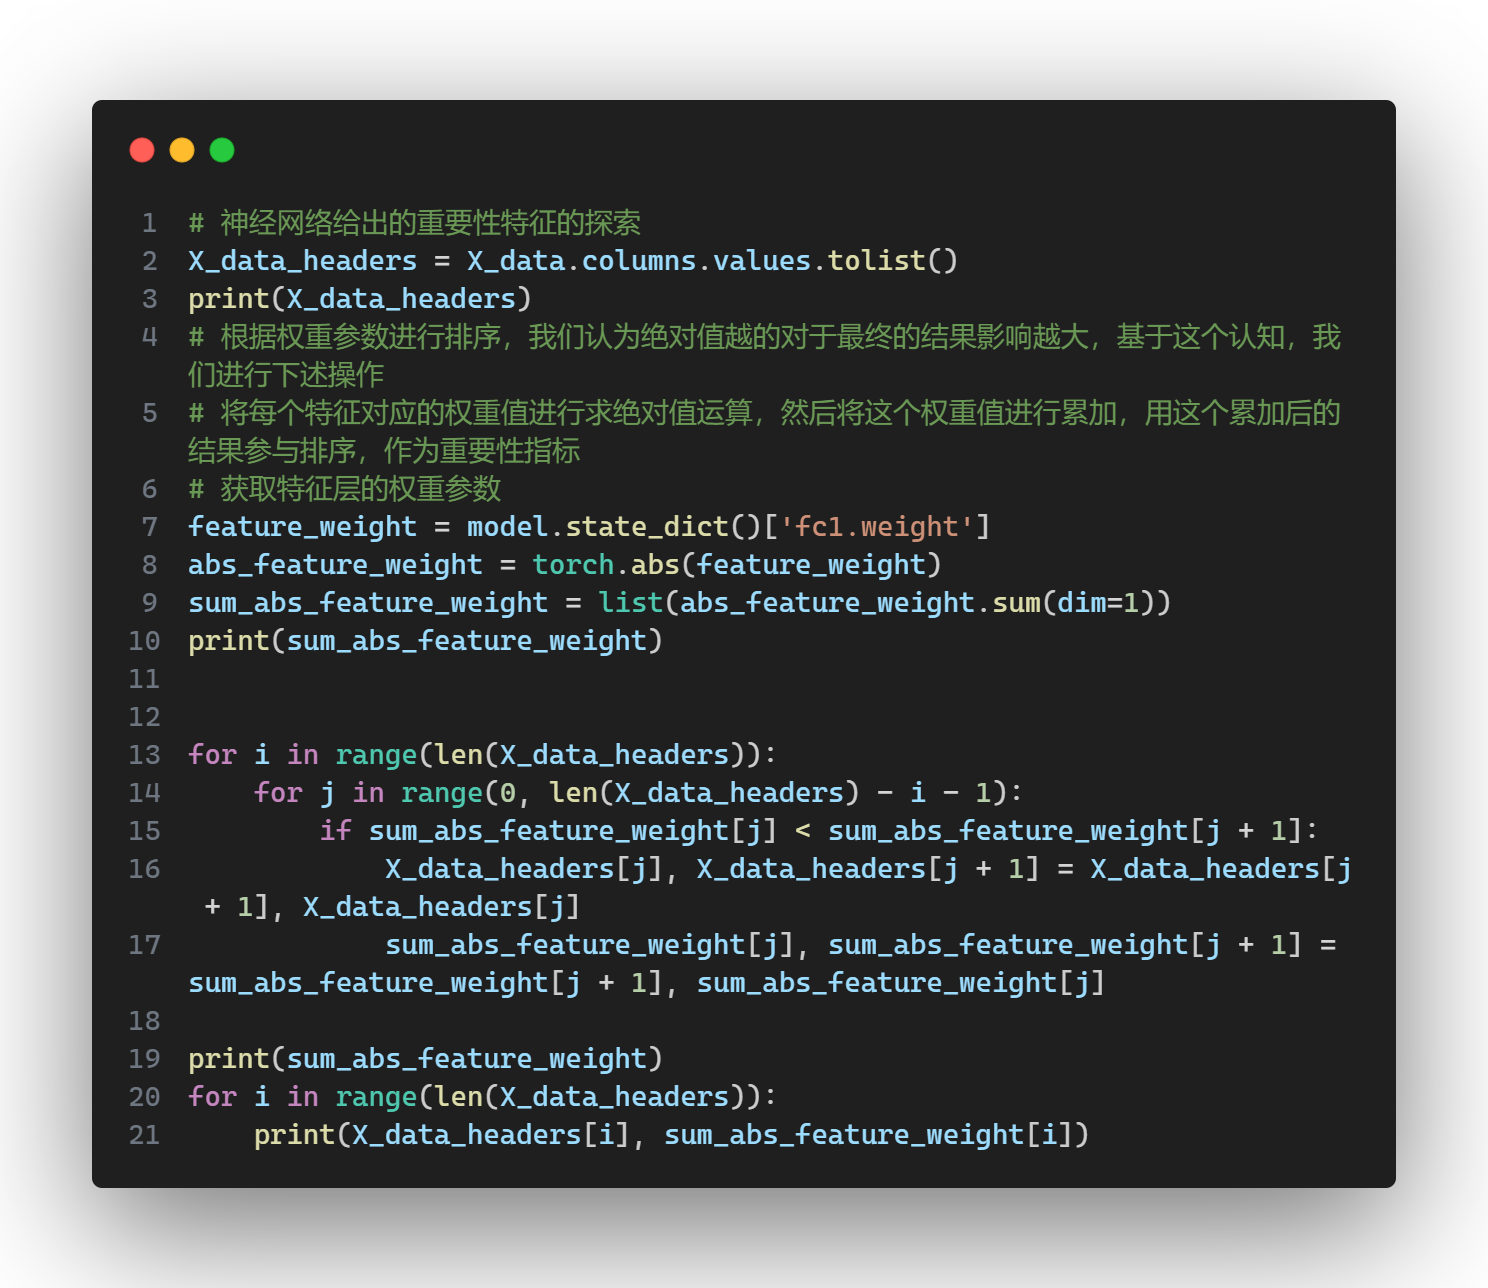
\includegraphics[width=\textwidth]{./img/mlp_f.png}
\end{figure}

根据权重参数进行排序,我们认为绝对值越的对于最终的结果影响越大,基于这个认知,我们进行下述操作:
\begin{itemize}
	\item 将每个特征对应的权重值进行求绝对值运算,然后将这个权重值进行累加,用这个累加后的结果参与排序,作为重要性指标
	\item 获取特征层的权重参数
	\item 根据这个值进行排序,给出如下结果
\end{itemize}
\begin{figure}[H]
	\centering
	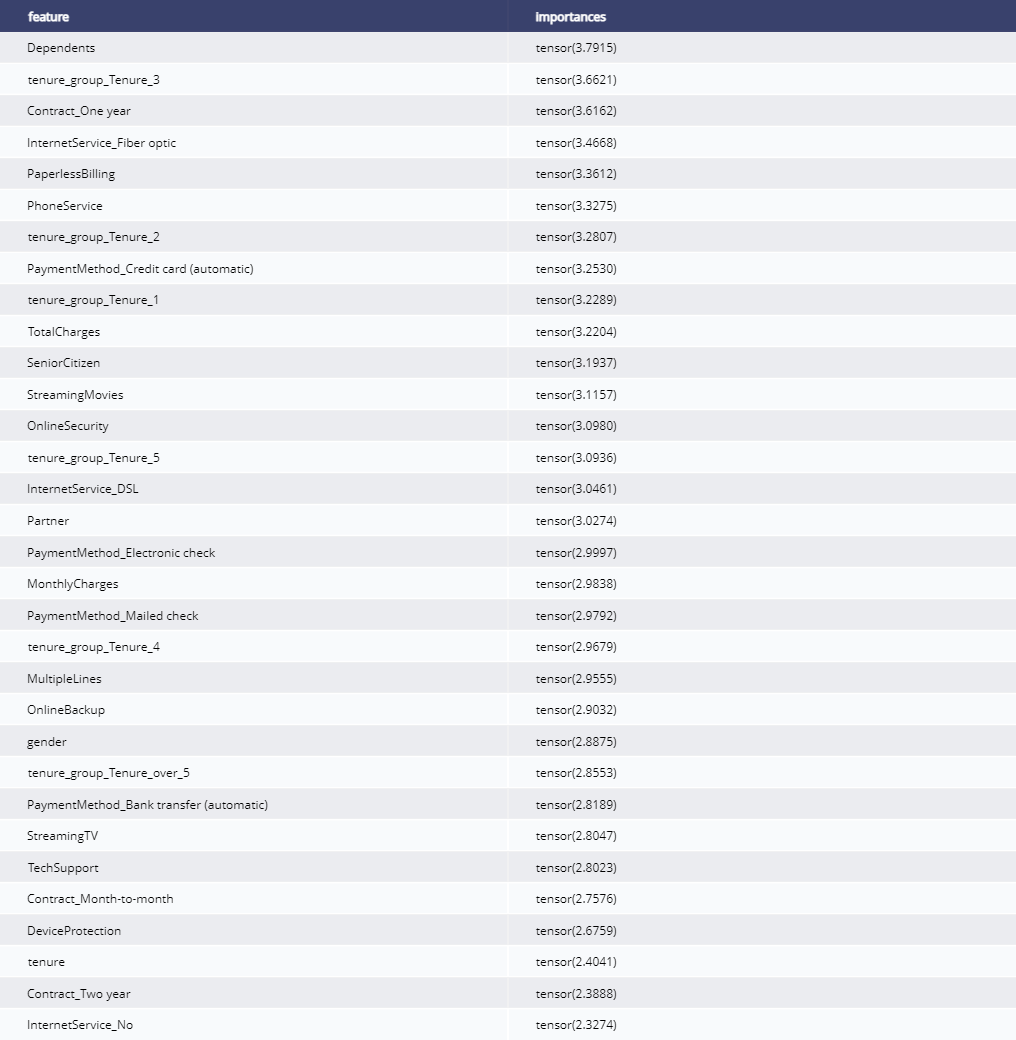
\includegraphics[width=\textwidth]{./img/mlp_res1.png}
\end{figure}
不足:上面的排序仅考虑了第一层提取特征层的权重,但是神经网络的结构不是这么简单的仅靠看第一层的权重就可以了解到特征的重要性的;而且这个累加的结果貌似快要出现了高位数据失效的情况,累加后趋近于同一个值的情况就要出现了,因此还有待改进,可以将第二层网络的维度减小进行再次的学习观察。
因此,为了验证我的这个思路是否正确,我重新跑了即便模型,分别记录他们给出的重要性排序,结果如下:

\begin{figure}[H]
	\centering
	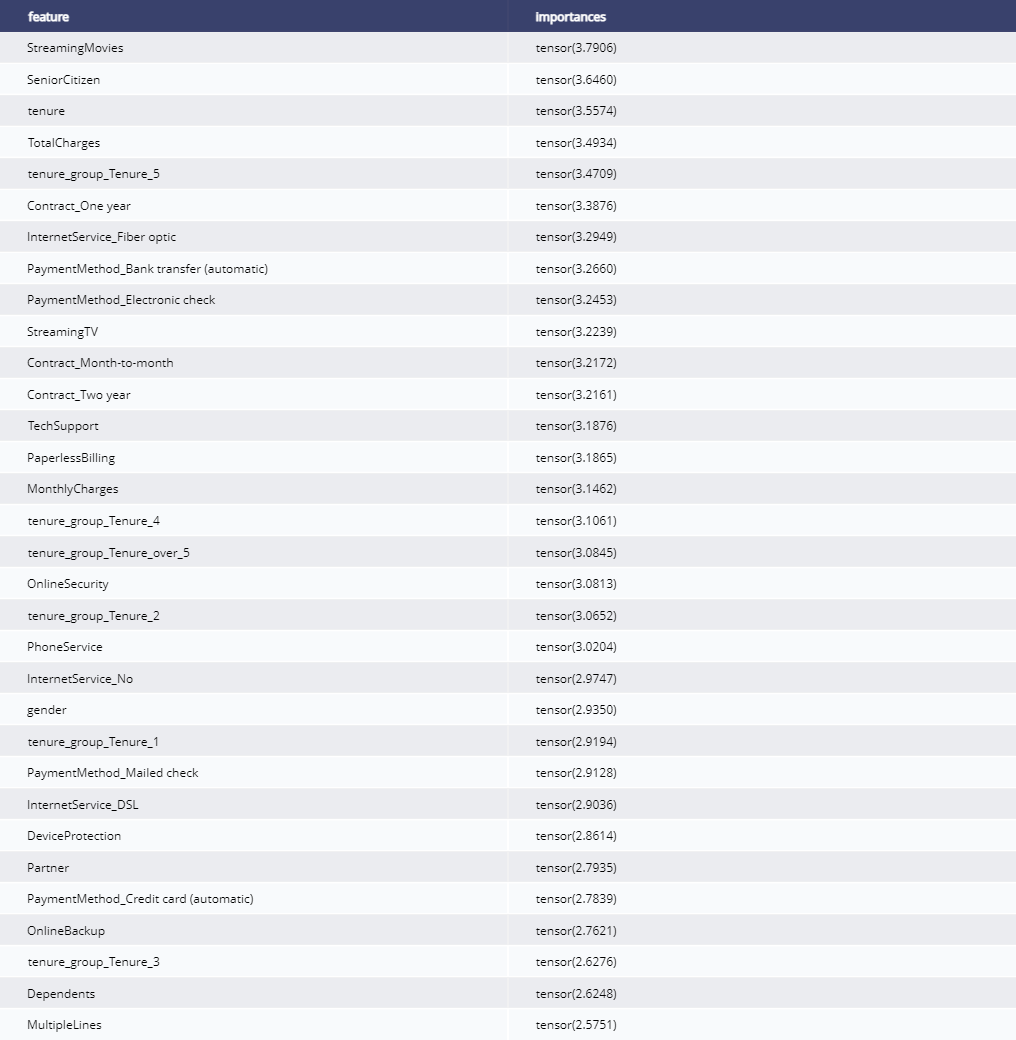
\includegraphics[width=\textwidth]{./img/mlp_res2.png}
\end{figure}

\begin{figure}[H]
	\centering
	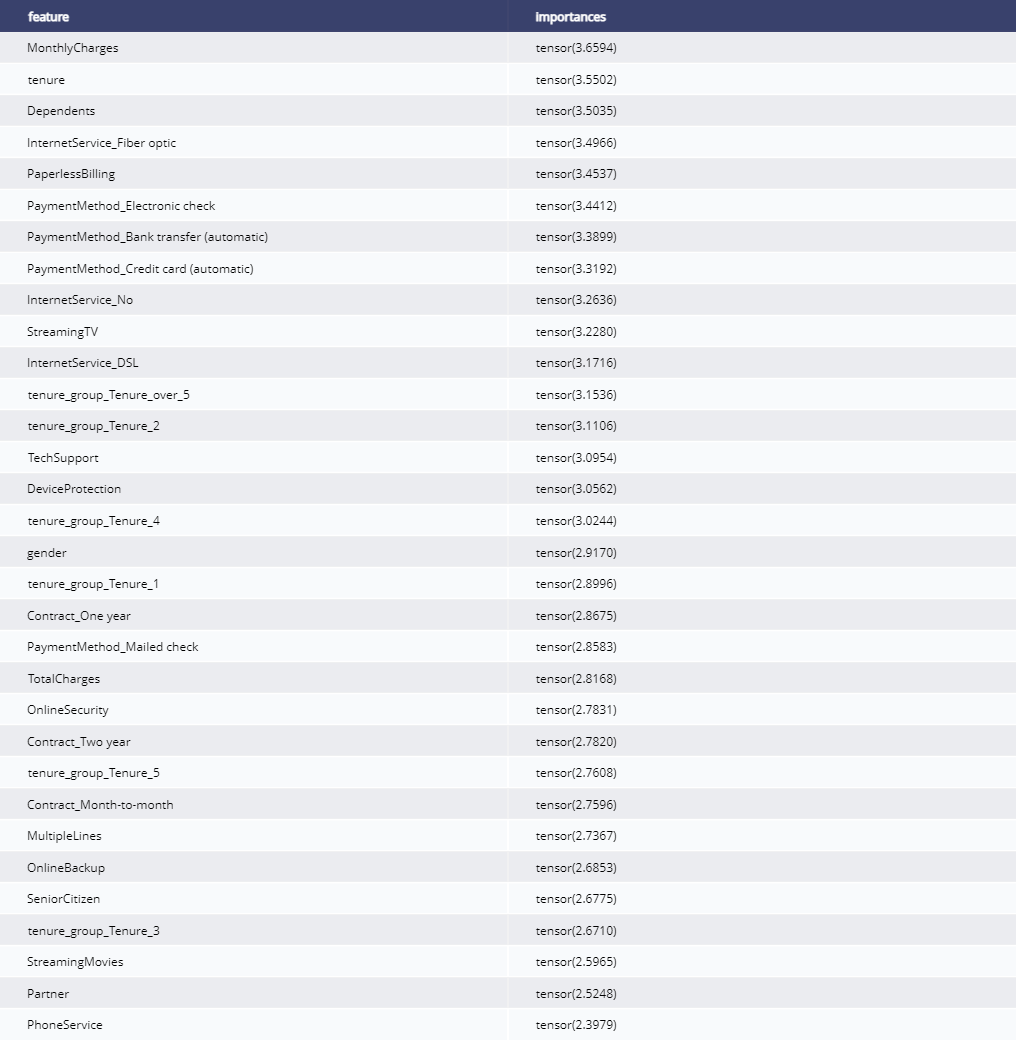
\includegraphics[width=\textwidth]{./img/mlp_res3.png}
\end{figure}
通过上述三个结果的对比,我发现使用这种方法给出的重要性排序具有很强的不确定性,初步断定是我们的测算方式导致的,因为这个方式没有考虑到整个网络里的参数传递,而且出现了高维数据的加和,因此不可靠,需要寻找其他办法给出特征重要性排序。

但是总的来说,这个方法去做预测是一个好的性能很好的模型,是一个成功的探索。

\subsection{模型评估总结}

最终我对比了所有实验效果,发现随机森林加上采样数据会实现最好的效果,因此最终部署的模型也将使用这个模型。

\section{模型的部署与分析}

这部分是为了完善整个业务流程,但实际上并没有真正实现,
部署即是把挖掘结果以要求的方式呈现给用户,本阶段要解决一些实际问题,
比如长期运行的模型是否有足够的机器来支撑,数据量以及并发程度会不会造成部署的服务器出现问题。
部署是一个挖掘项目的结束,也是一个数据挖掘项目的开始。

\section{实验小结}

本实验是在老师提供的baseline的基础上做进一步的性能提升,尝试更多的方法,体会数据挖掘过程的整个流程,这部分主要由baseline给的思路和上课所学了解到,
本人在实验主要贡献有以下几个方面:

\subsection{工程方面}

\begin{itemize}
	\item 在与在baseline的基础上将整个流程用markdown的标题重构组织了一遍,使得整个流程的数据流更加清晰规范,之后想要扩展这个流程的话只需要在相应的模块进行更改即可,提升了代码的可读性和友好性
	\item 将各种经过不同操作处理的数据进行了分别保存和规范命名,方便后续实验和后人使用,也方便加入新的数据处理方式
	\item 对使用不同的模型和数据的情况进行了多种实验,筛选出了baseline中最好数据挖掘效果的模型
\end{itemize}

\subsection{算法方面}

\begin{itemize}
	\item 数据压缩方面,我加入了PCA主成分分析方法的数据压缩,评测了数据降维的效果,发现各种降维的方式在这个业务数据背景中效果并不好,有负面的影响,因此将baseline中的特征检定筛选模块剔除了
	\item 将10折交叉验证封装进了原本代码中的report\_model函数中,提高了模型评估的公平性,消除了偶然性
	\item 使用上采样流失客户数据的方式解决了数据不平衡的问题,使得模型效果有了很大的提升
	\item 自己实现了决策树模型的集成过程
	\item 决策树调参(baseline中已有)
	\item 自己实现了MLP算法并在数据上进行了测评取得了较好的效果
\end{itemize}

以上就是实验的所有内容。

\bibliographystyle{unsrt}      %参考文献样式
\bibliography{D:/Data/paper_database/better-bibtex/refe}  

\end{document}
